Die deskriptive Auswertung basiert auf dem finalen Roman-Panel vom 1. August 2024 bis zum 30. Juni 2026.  Damit enthält der Analysedatensatz 1.316 tatsächliche Haushalte: 61 Kontrollhaushalte, 121 Haushalte im statischen Tarifarm und 125 Haushalte im dynamischen Tarifarm in Linz Netz (LN) sowie 514 Kontroll- und 495 Tarifhaushalte in Netz Oberösterreich (NOÖ). Der Beginn der Tarifphase ist der 1. August 2025.

Der Kerndatensatz enthält Viertelstundenwerte zu Netzbezug, Netzeinspeisung und Nettolast sowie Tarifsignale und Tarifkomponenten. Der Netzbezug wird im Folgenden als Verbrauch bezeichnet. Die Einspeisung misst nur die tatsächlich in das Netz abgegebene Energie und ist daher nicht identisch mit der gesamten PV-Erzeugung eines Haushalts.

\subsection{Verteilung der Viertelstundenwerte}

Bevor die zeitlichen Muster betrachtet werden, ist die Verteilung der Messwerte selbst wichtig. Abbildung~\ref{fig:report_consumption_15m_density} zeigt die Verteilung des Netzbezugs auf Viertelstundenebene. Die Dichte ist stark am unteren Rand konzentriert und weist gleichzeitig einen langen rechten Rand auf. Das bedeutet: Ein großer Teil der Viertelstundenwerte ist sehr klein oder null, während einzelne Intervalle deutlich höhere Lasten aufweisen. Diese Struktur ist typisch für Haushaltslastdaten, aber für einfache lineare Modelle mit homoskedastischen und annähernd normalverteilten Fehlern ungünstig.

\begin{figure}[H]
    \centering
    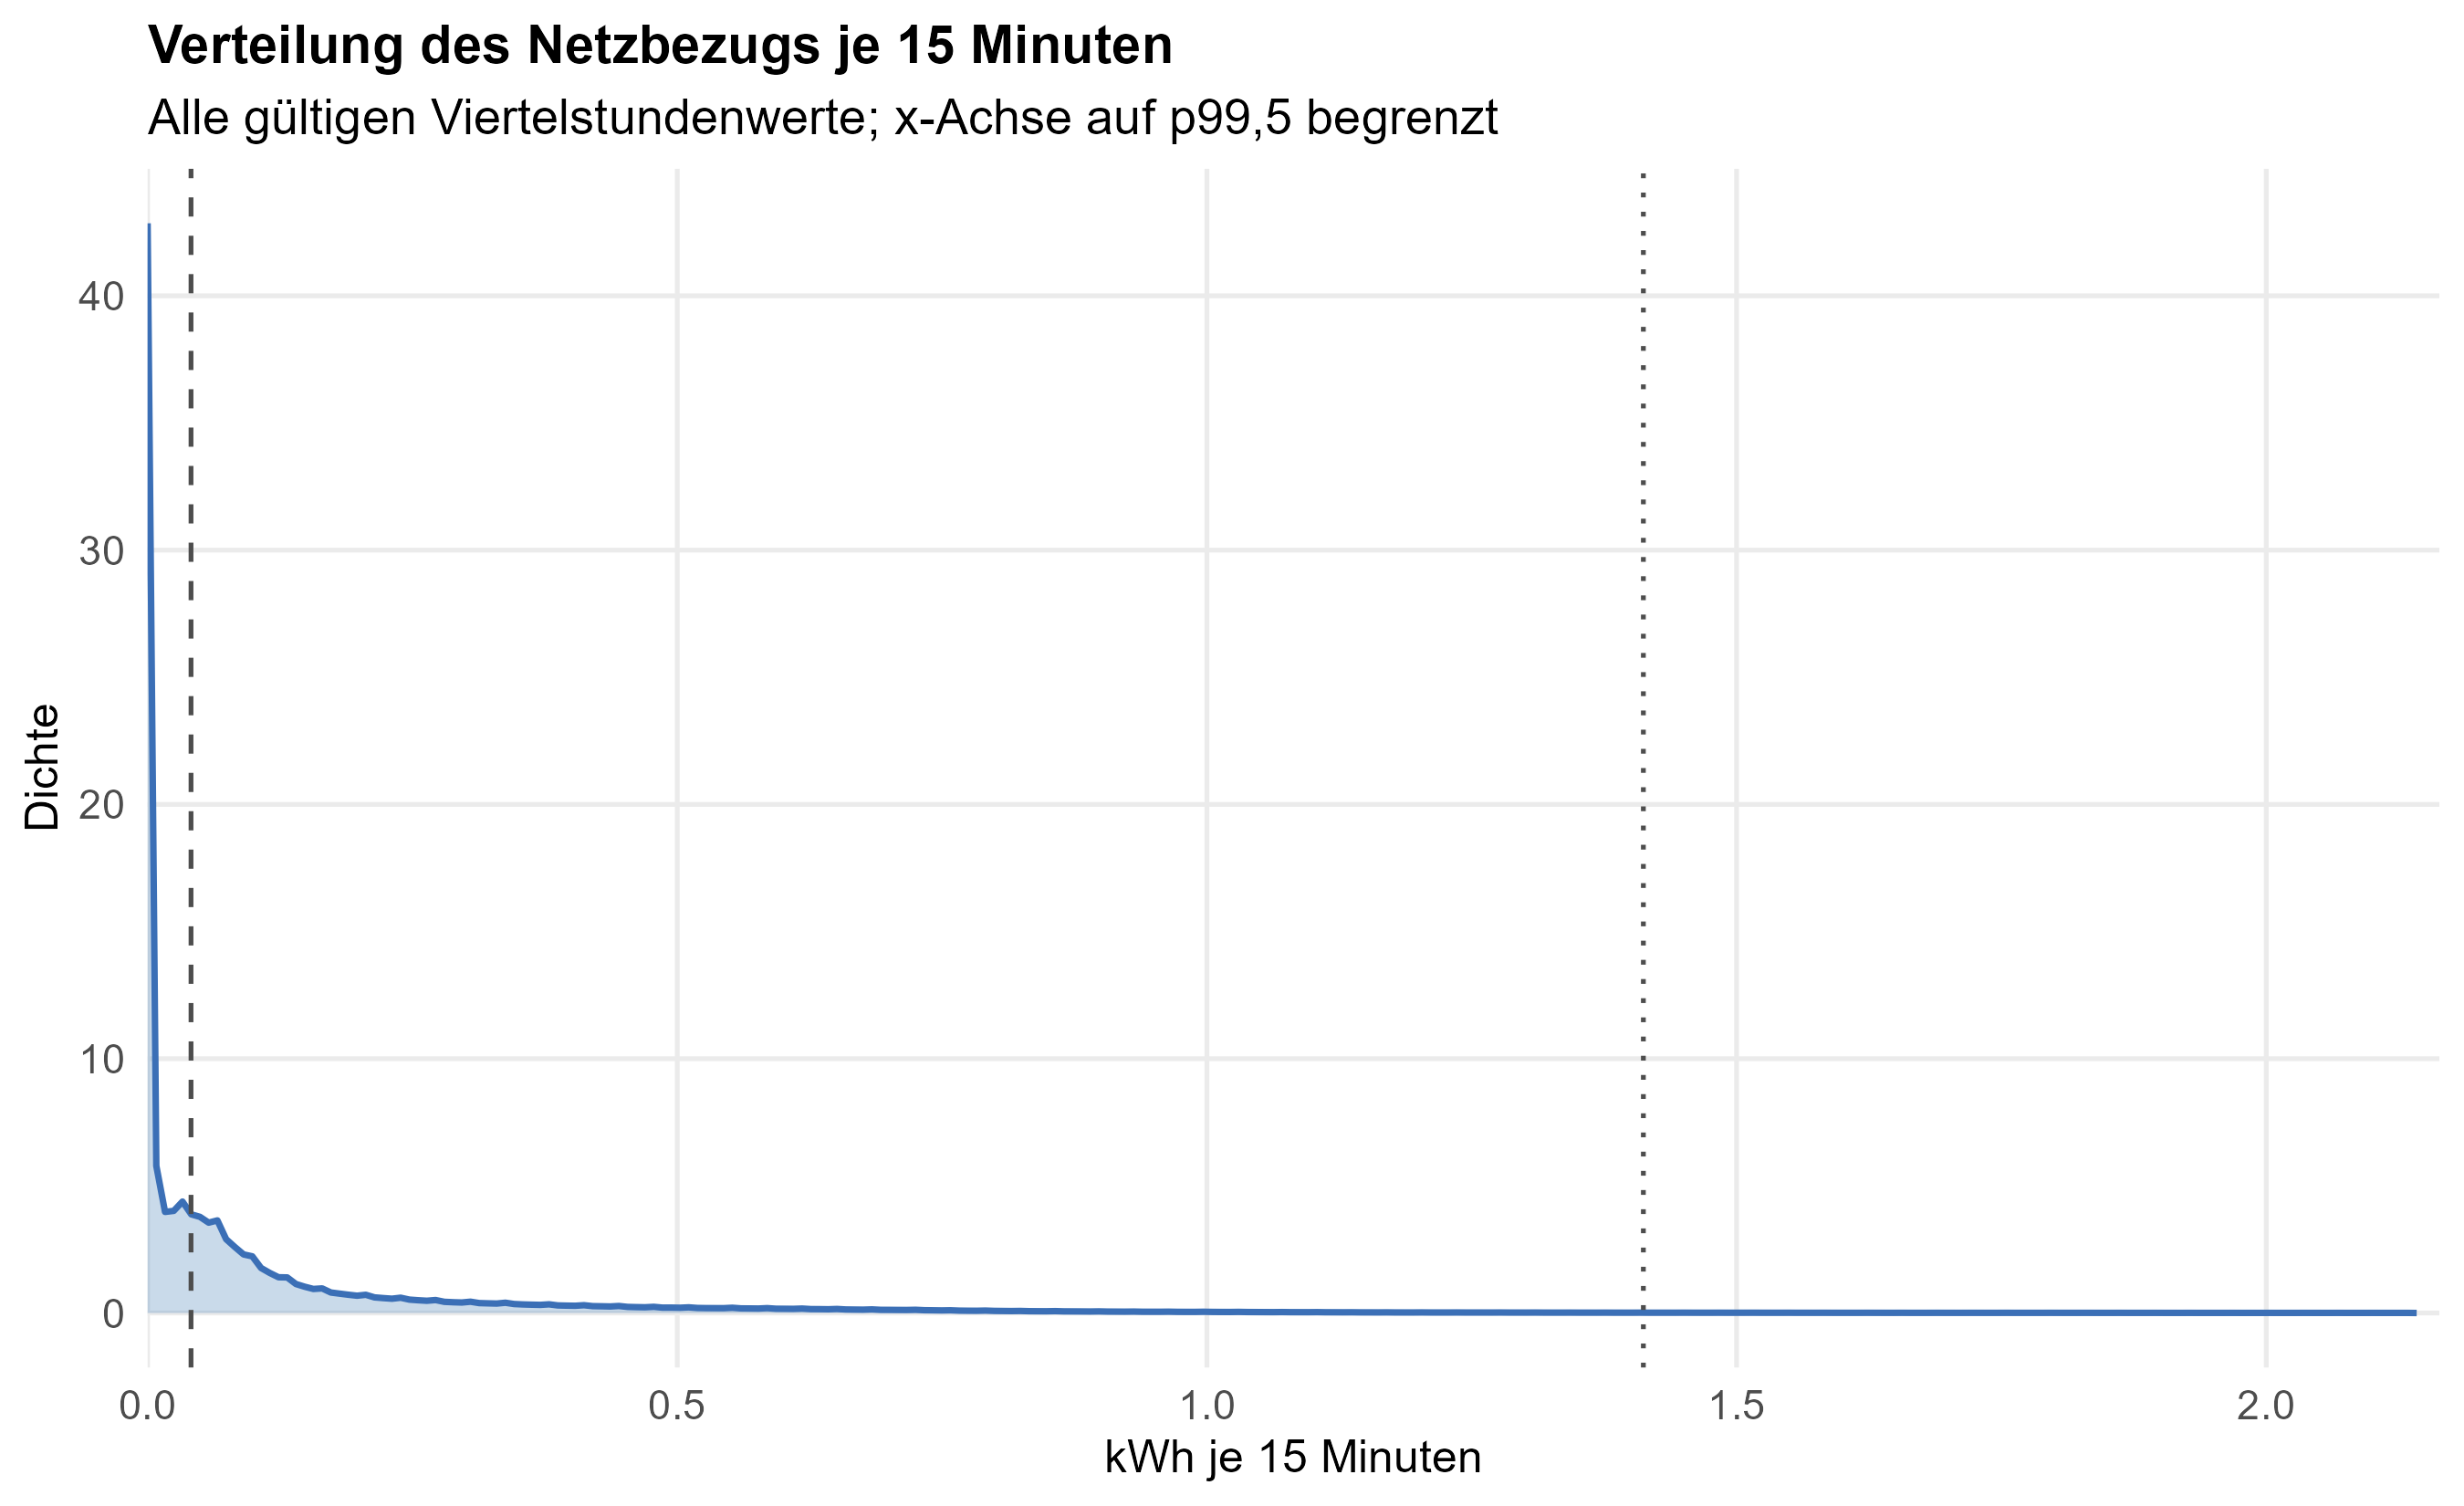
\includegraphics[width=0.92\linewidth]{paper/figures/report_fig00_consumption_15m_density.png}
    \caption{Verteilung des Netzbezugs je 15 Minuten. Das Histogramm ist als Dichte skaliert; die gestrichelte Linie markiert den Median, die gepunktete Linie das 99. Perzentil.}
    \label{fig:report_consumption_15m_density}
\end{figure}

Tabelle~\ref{tab:consumption_15m_distribution} fasst dieselbe Verteilung numerisch zusammen. In allen Untersuchungsgruppen liegt der Median deutlich unter dem Mittelwert, und die oberen Perzentile liegen um ein Vielfaches über dem typischen Viertelstundenwert. Diese Schiefe ist ein zentraler Grund, weshalb die kausale Hauptspezifikation später als Poisson-Pseudo-Maximum-Likelihood-Modell geschätzt wird. OLS bleibt als ergänzende Spezifikation für absolute Effekte in kWh hilfreich, ist aber nicht die natürlichste Hauptspezifikation für die Viertelstundenlast.

\begin{table}[H]
\centering
\caption{Verteilung des Netzbezugs auf Viertelstundenebene}
\label{tab:consumption_15m_distribution}
\begin{tabular}{lrrrrrrr}
\toprule
Gruppe & $N$ (Mio.) & Nullanteil & Mittelwert & Median & p90 & p99 & p99,5 \\
\midrule
Gesamt & 84.4 & 15.6\% & 0.143 & 0.041 & 0.405 & 1.412 & 2.142 \\
LN Kontroll & 3.7 & 16.4\% & 0.111 & 0.032 & 0.295 & 1.209 & 1.609 \\
LN Dynamisch & 7.8 & 15.0\% & 0.112 & 0.034 & 0.296 & 1.119 & 1.661 \\
LN Statisch & 7.5 & 16.2\% & 0.139 & 0.036 & 0.384 & 1.529 & 2.426 \\
NOÖ Kontroll & 33.0 & 15.2\% & 0.147 & 0.046 & 0.423 & 1.363 & 1.977 \\
NOÖ Tarif & 32.4 & 15.9\% & 0.152 & 0.042 & 0.429 & 1.541 & 2.441 \\
\bottomrule
\end{tabular}
\begin{flushleft}
\footnotesize Werte in kWh je 15 Minuten. Fehlende Werte sind ausgeschlossen.
\end{flushleft}
\end{table}


\subsection{Verbrauch, Einspeisung und Kosten im Zeitverlauf}

Abbildung~\ref{fig:report_daily_consumption_feedin} zeigt den durchschnittlichen täglichen Netzbezug und die durchschnittliche tägliche Netzeinspeisung je Haushalt. Die Werte werden zunächst je Haushalt und Tag summiert und anschließend innerhalb der jeweiligen Untersuchungsgruppe gemittelt. In NOÖ liegen Tarif- und Kontrollgruppe im Verbrauch über weite Teile des Beobachtungszeitraums nahe beieinander. In LN verlaufen Kontrollgruppe und dynamischer Tarifarm nahezu deckungsgleich, während der statische Tarifarm bereits vor Tarifbeginn auf einem sichtbar höheren Niveau liegt. Die Einspeisung ist deutlich saisonal geprägt und konzentriert sich erwartungsgemäß auf Frühjahr und Sommer.

\begin{figure}[H]
    \centering
    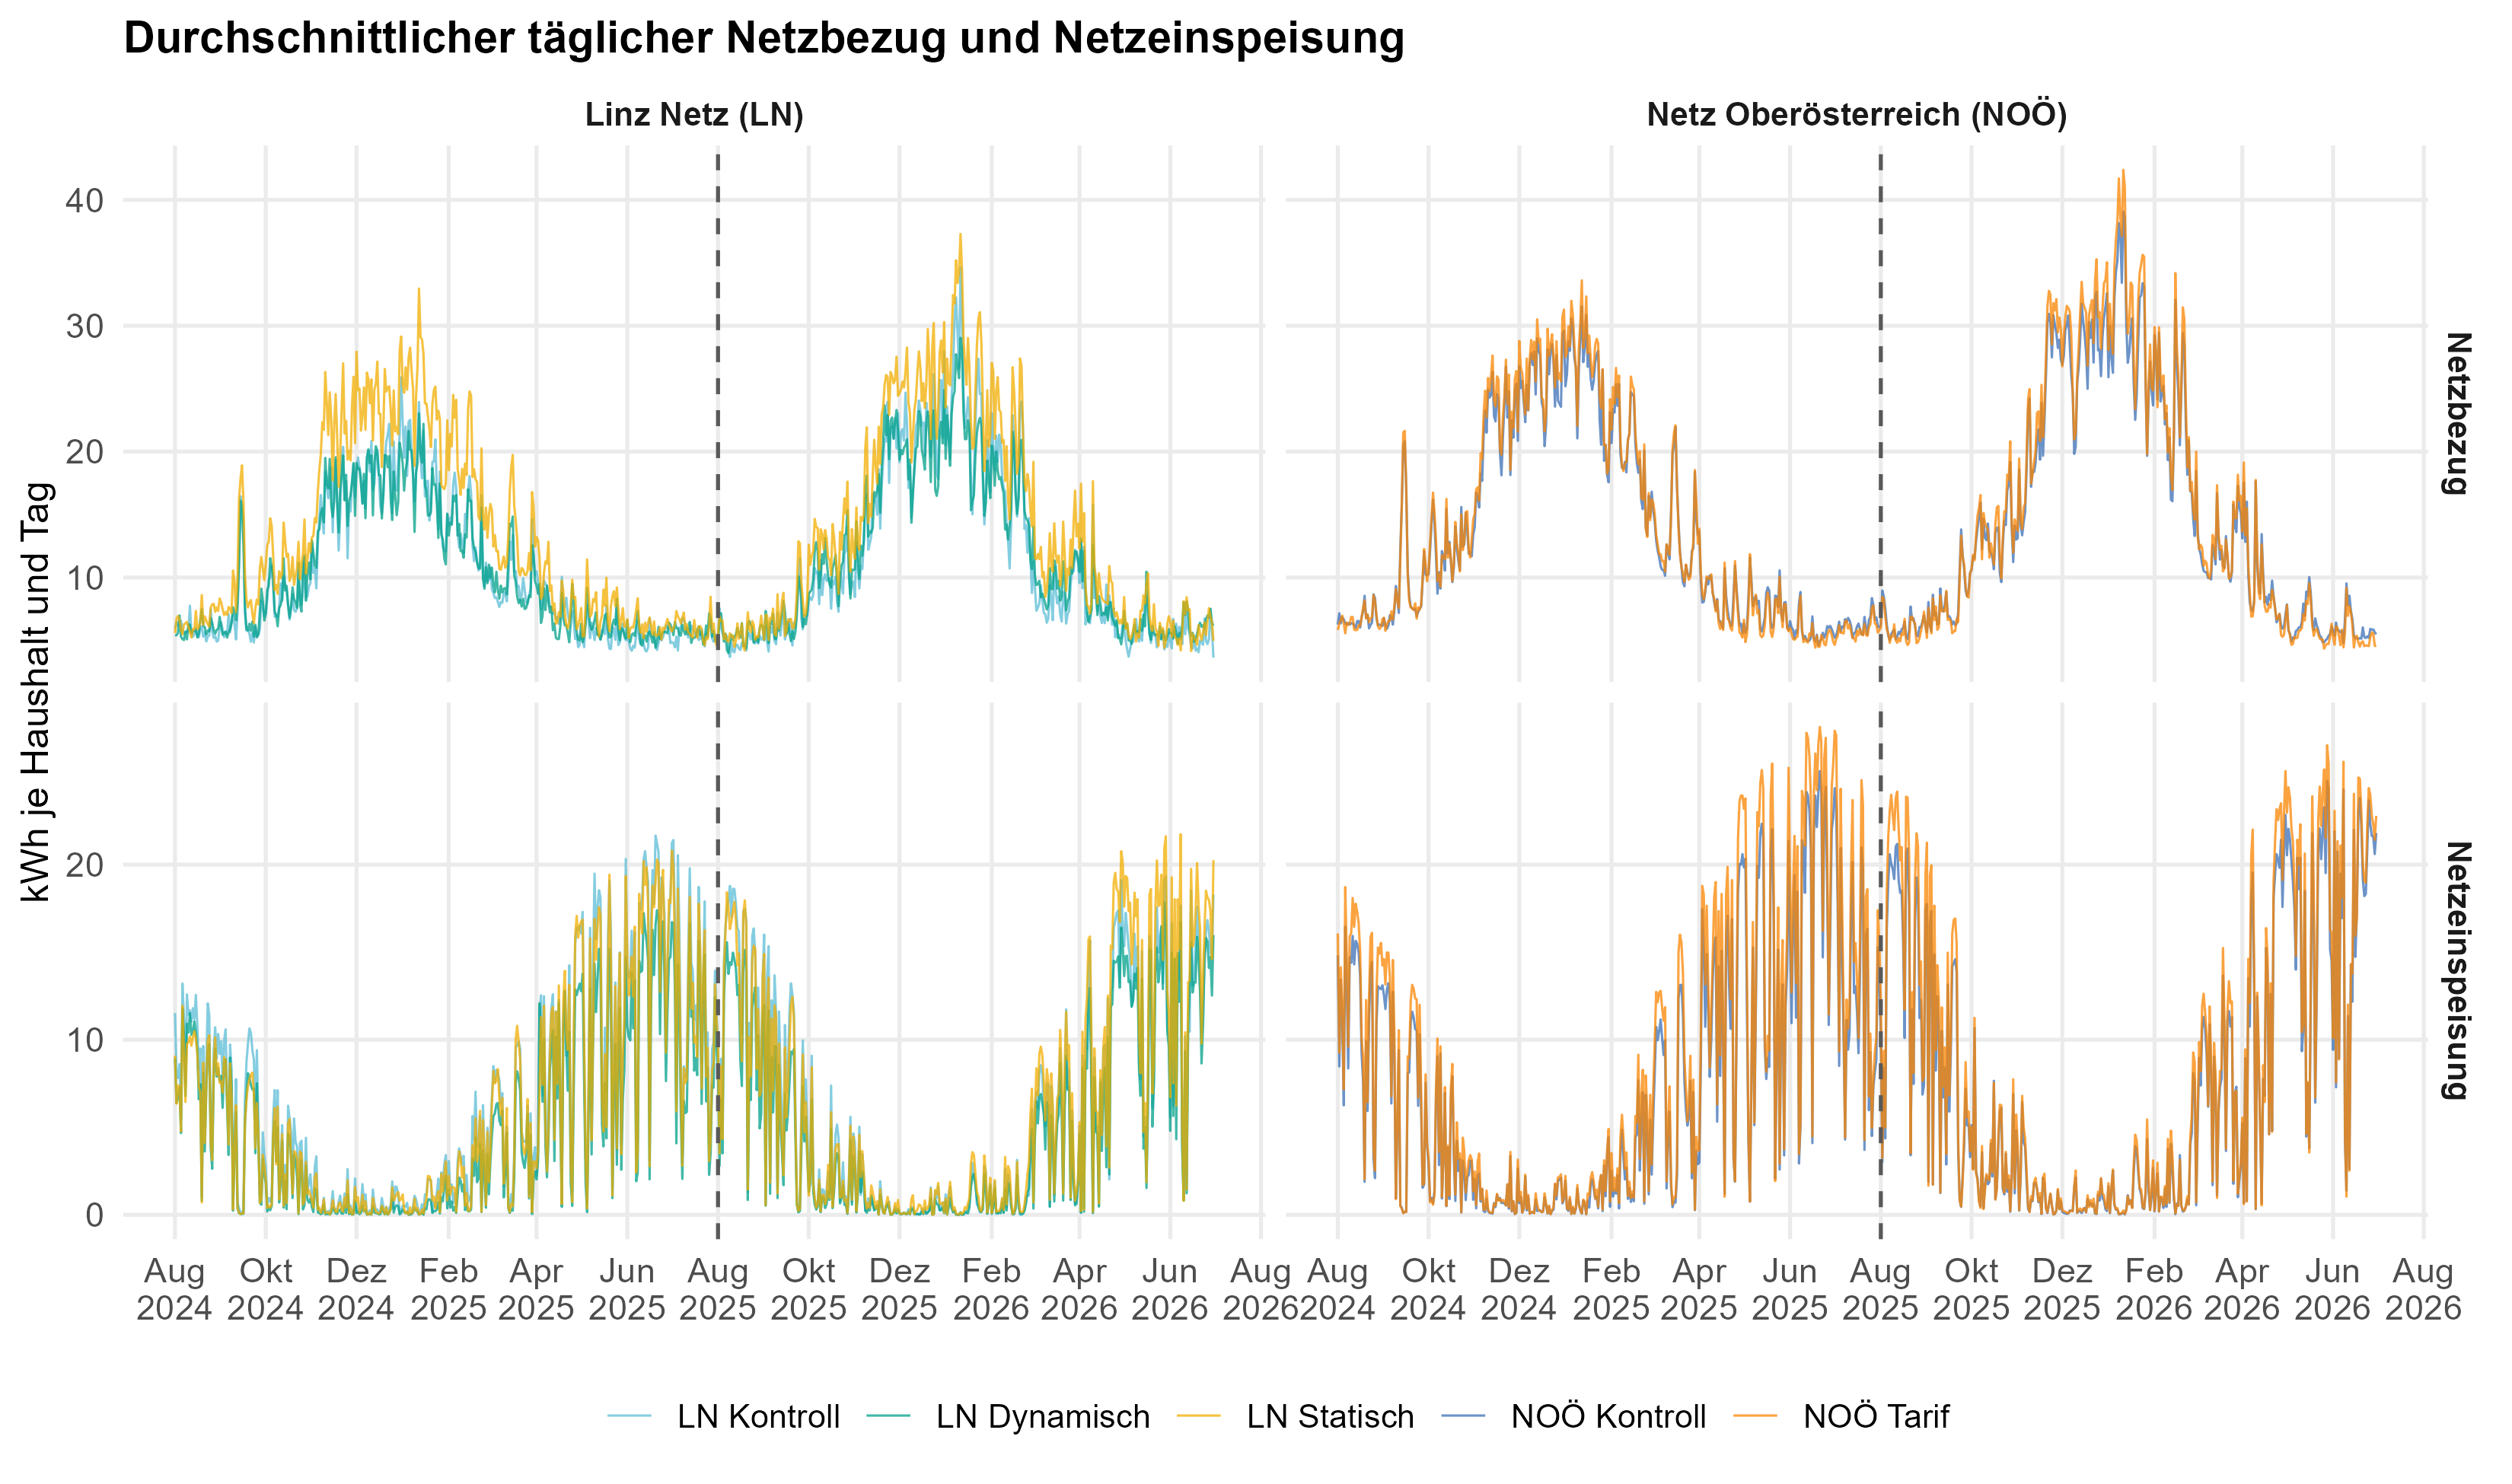
\includegraphics[width=1\linewidth]{paper/figures/report_fig01_daily_consumption_feedin.png}
    \caption{Durchschnittlicher täglicher Netzbezug und durchschnittliche tägliche Netzeinspeisung je Haushalt. Die gestrichelte Linie markiert den Beginn der Tarifphase am 1. August 2025.}
    \label{fig:report_daily_consumption_feedin}
\end{figure}

Abbildung~\ref{fig:report_financial_timeseries} ordnet dieselben Verbrauchsdaten monetär ein. Dargestellt sind variable Energie- und Netzkosten auf Basis des Viertelstundenbezugs und der im Datensatz hinterlegten Tarifkomponenten. Die Werte sind keine vollständige Haushaltsrechnung: Grundpreise, Steuern, Abgaben und individuelle Vertragsdetails werden nicht abgebildet. Für LN ist die Darstellung zusätzlich vorsichtig zu interpretieren, weil der eigentliche Netztarif peak-basiert ist und nicht vollständig durch eine einfache Viertelstundenmultiplikation beschrieben wird.

\begin{figure}[H]
    \centering
    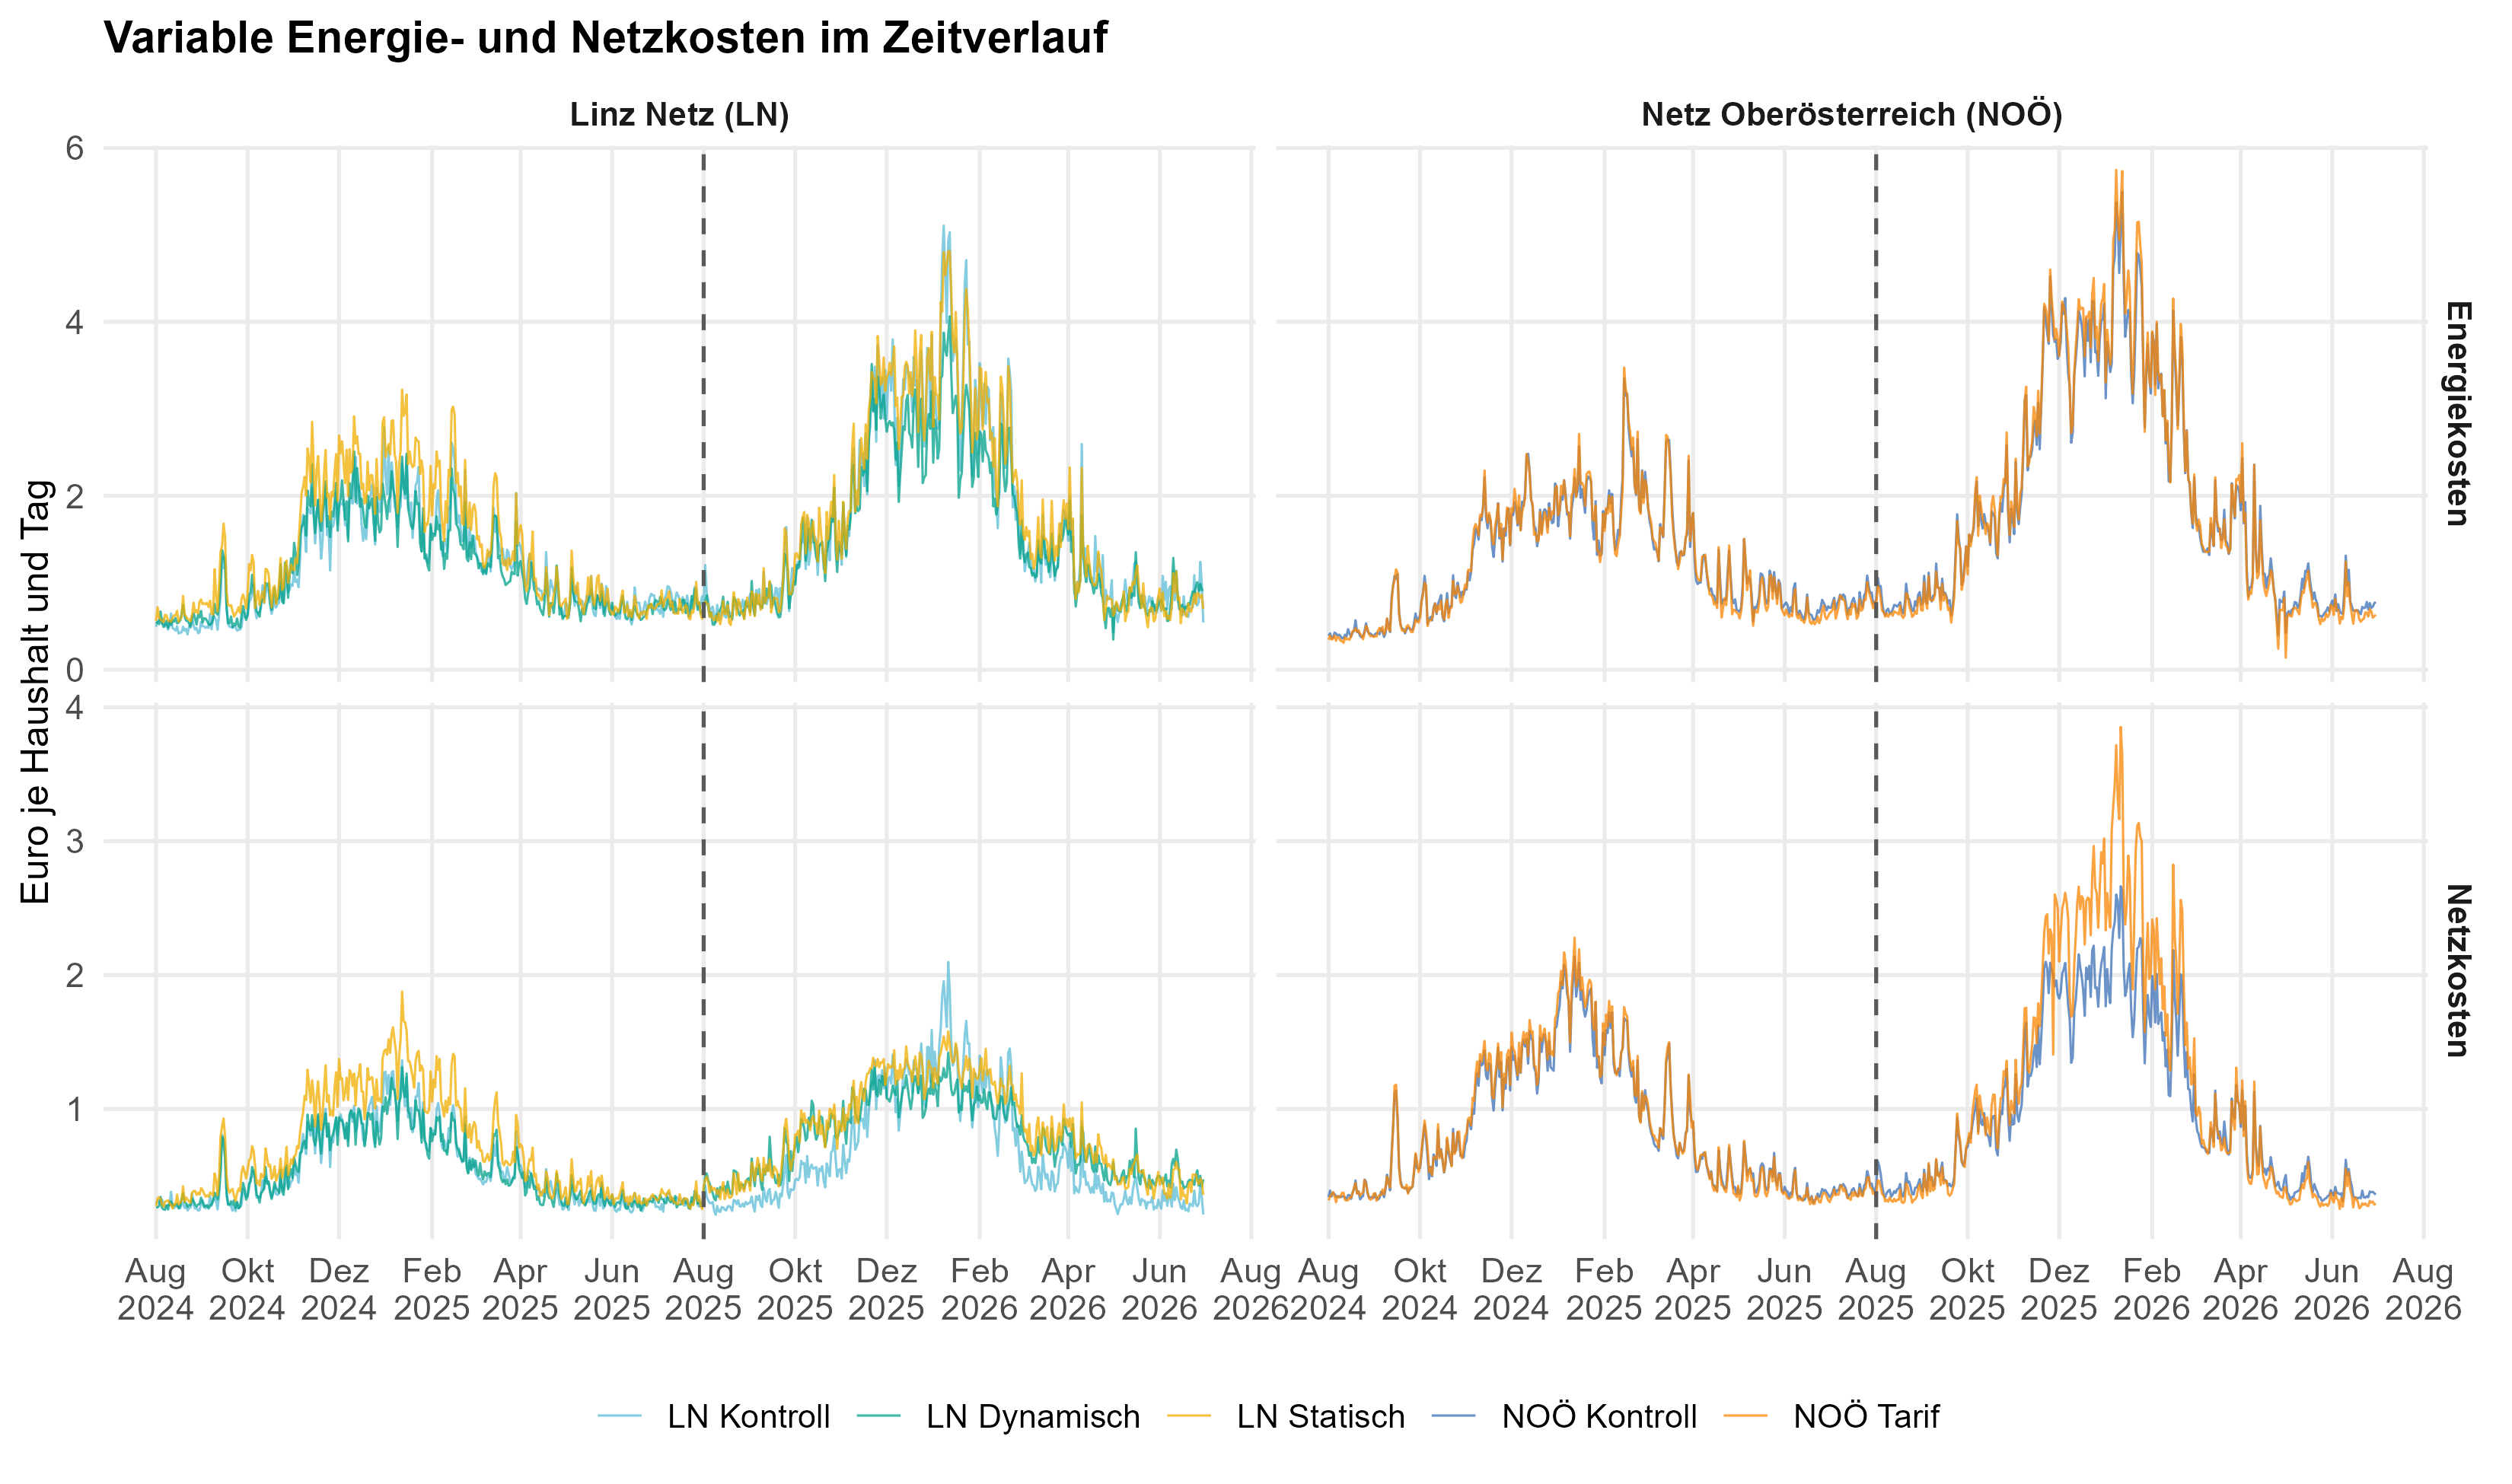
\includegraphics[width=1\linewidth]{paper/figures/report_fig02_financial_timeseries.png}
    \caption{Variable Energie- und Netzkosten je Haushalt und Tag. Die Berechnung approximiert variable Kosten als Viertelstundenbezug multipliziert mit dem jeweiligen Energie- beziehungsweise Netztarif.}
    \label{fig:report_financial_timeseries}
\end{figure}

\subsection{Spitzenlasten und typische Tagesprofile}

Abbildung~\ref{fig:report_daily_peaks} zeigt die durchschnittliche tägliche Spitzenlast. Dazu wird für jeden Haushalt und Tag die höchste Viertelstundenlast bestimmt; Viertelstundenwerte in kWh werden dafür in durchschnittliche Leistung umgerechnet (\(\text{kW} = \text{kWh}_{15\text{min}} \times 4\)). Anschließend wird der Mittelwert je Gruppe gebildet. Die Spitzenlasten folgen einem klaren saisonalen Muster und steigen in den Wintermonaten deutlich an. Für LN ist erneut sichtbar, dass der statische Tarifarm bereits vor der Intervention auf einem höheren Niveau liegt als Kontrollgruppe und dynamischer Arm.

\begin{figure}[H]
    \centering
    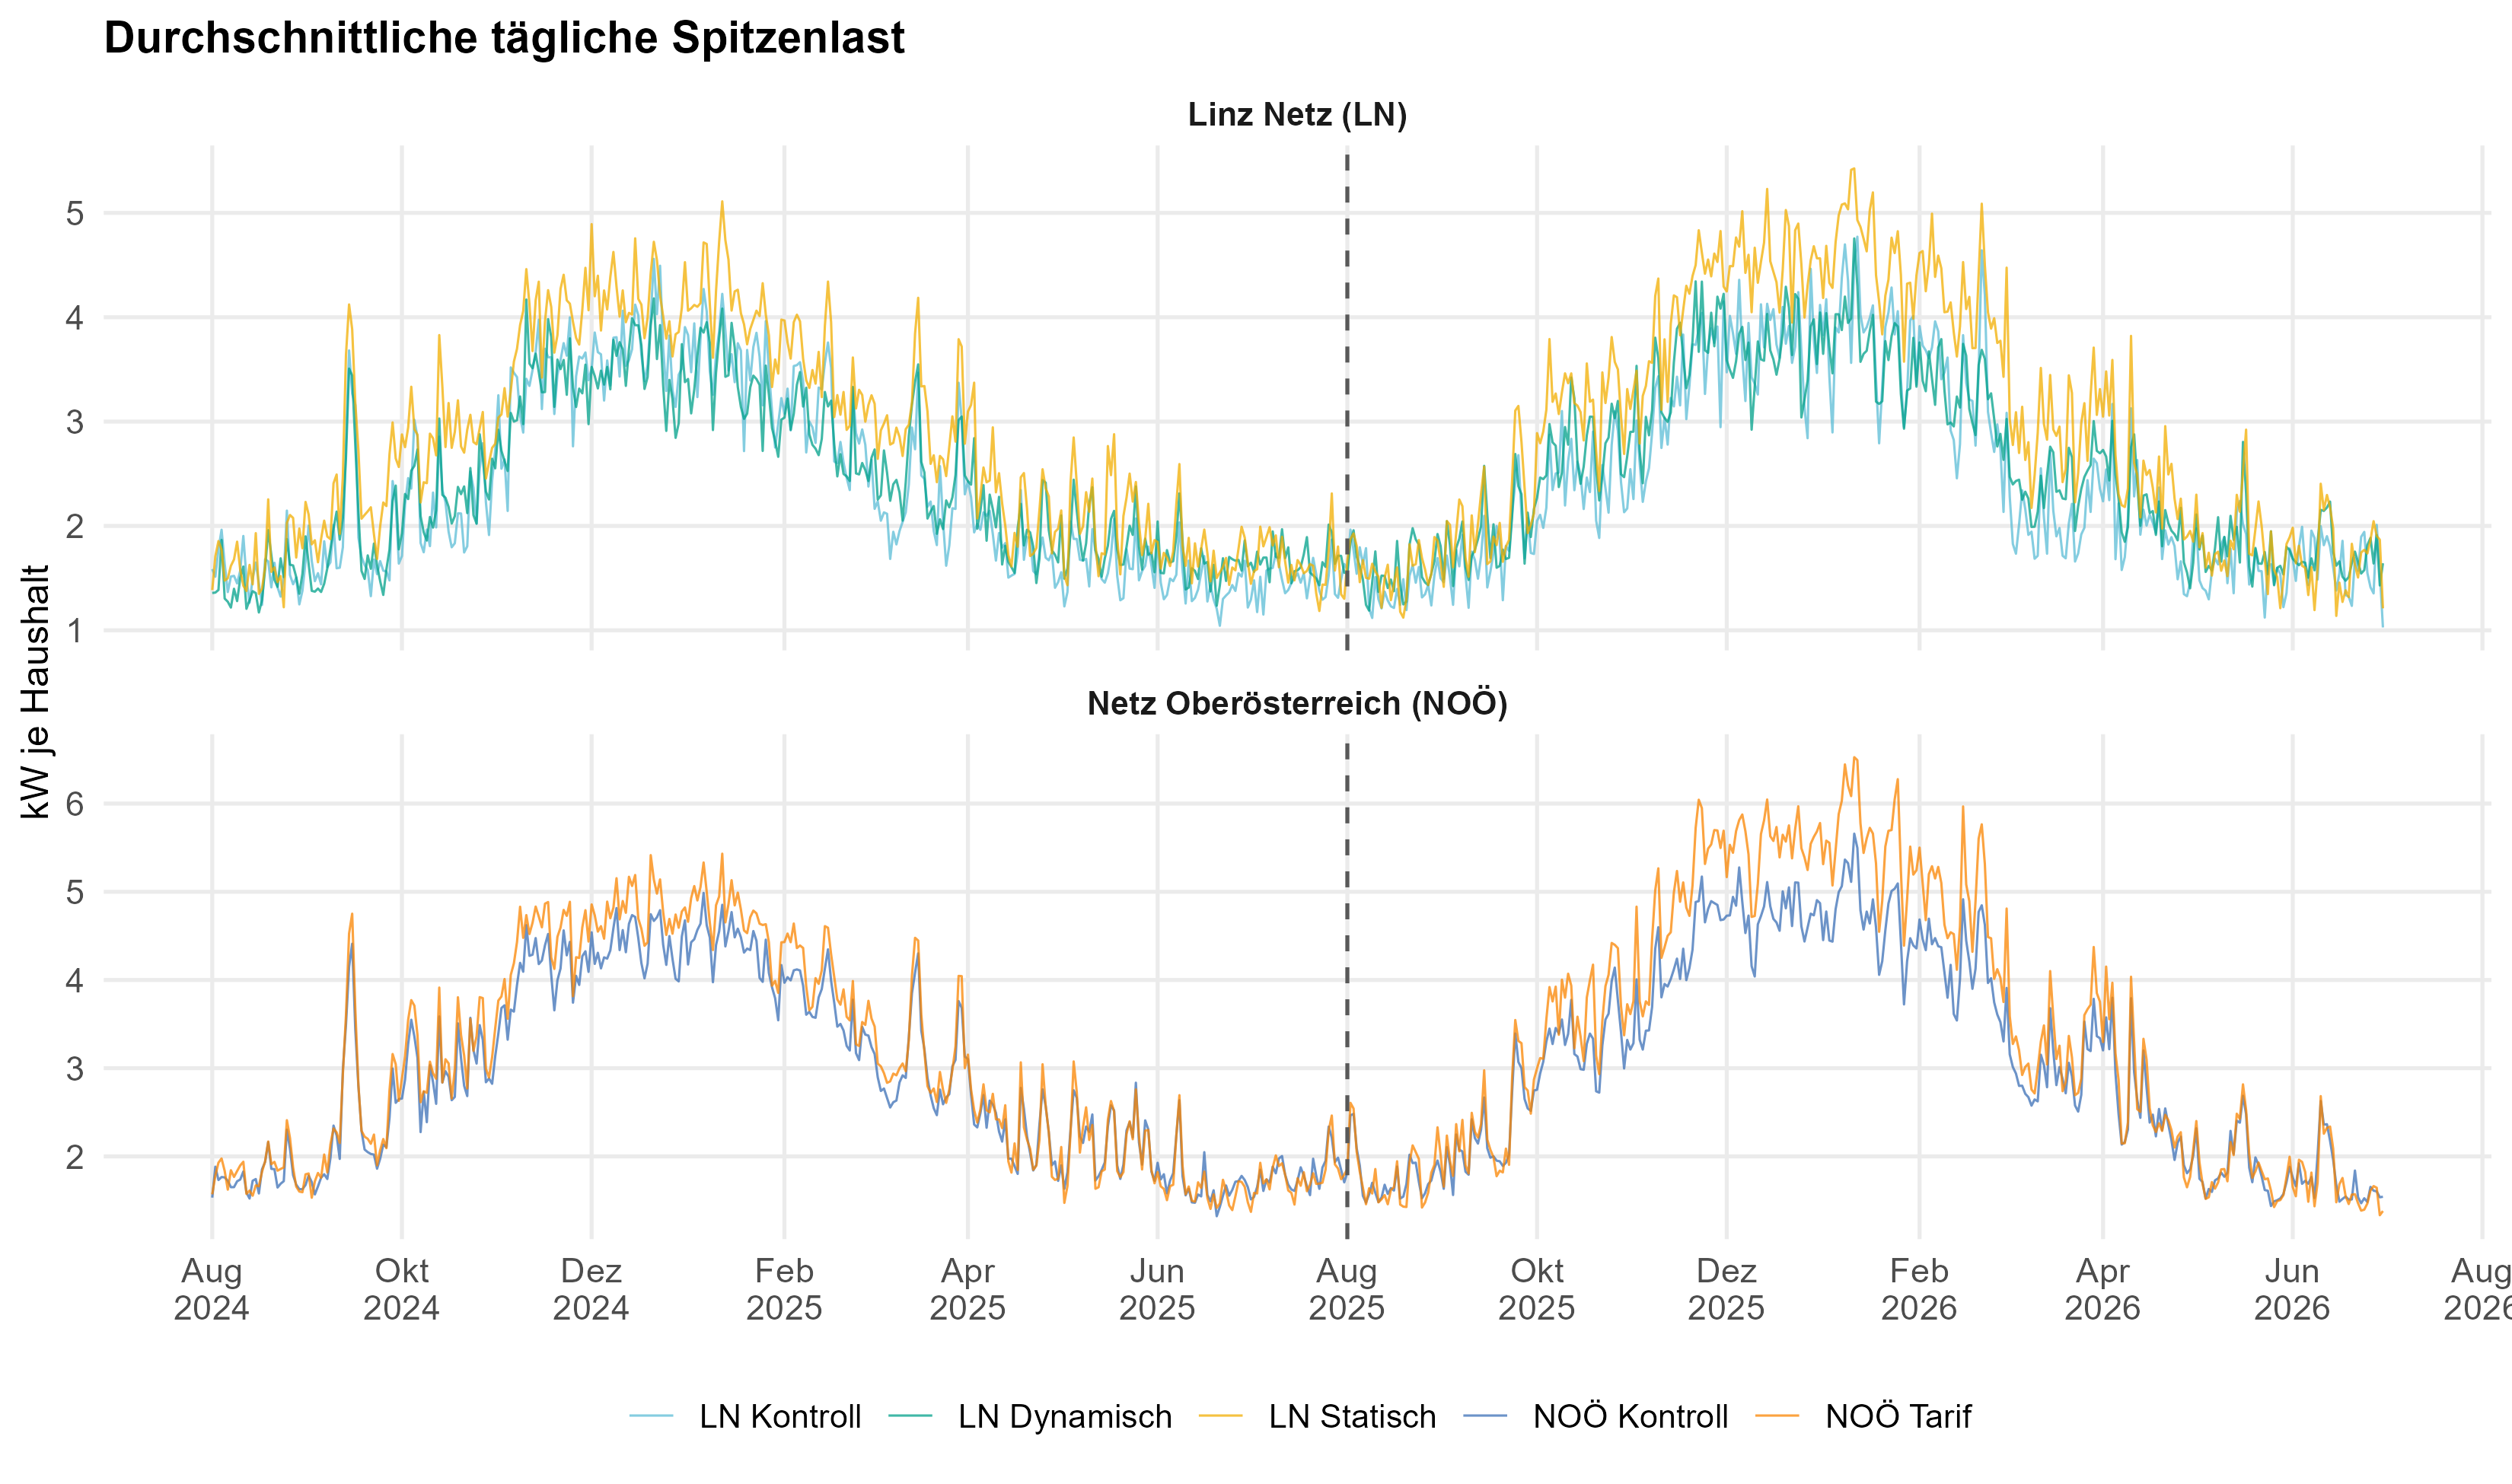
\includegraphics[width=1\linewidth]{paper/figures/report_fig03_daily_peaks.png}
    \caption{Durchschnittliche tägliche Spitzenlast je Haushalt. Die Spitzenlast ist das Maximum der Viertelstundenleistung eines Haushalts an einem Tag.}
    \label{fig:report_daily_peaks}
\end{figure}

Abbildung~\ref{fig:report_seasonal_profiles} zeigt typische 24-Stunden-Profile vor Beginn der Tarifphase, getrennt nach meteorologischen Jahreszeiten und danach, ob ein Haushalt eine PV-Anlage beziehungsweise einen Einspeisekanal aufweist. Die Profile basieren ausschließlich auf der Vorperiode vom 1. August 2024 bis zum 31. Juli 2025, damit die dargestellten Muster nicht durch mögliche Tarifeffekte beeinflusst werden. Die Trennung nach PV-Status ist wichtig, weil PV-Haushalte durch Eigenverbrauch und Einspeisung insbesondere um die Mittagszeit ein anderes Bezugsprofil aufweisen können als Haushalte ohne PV.

\begin{figure}[H]
    \centering
    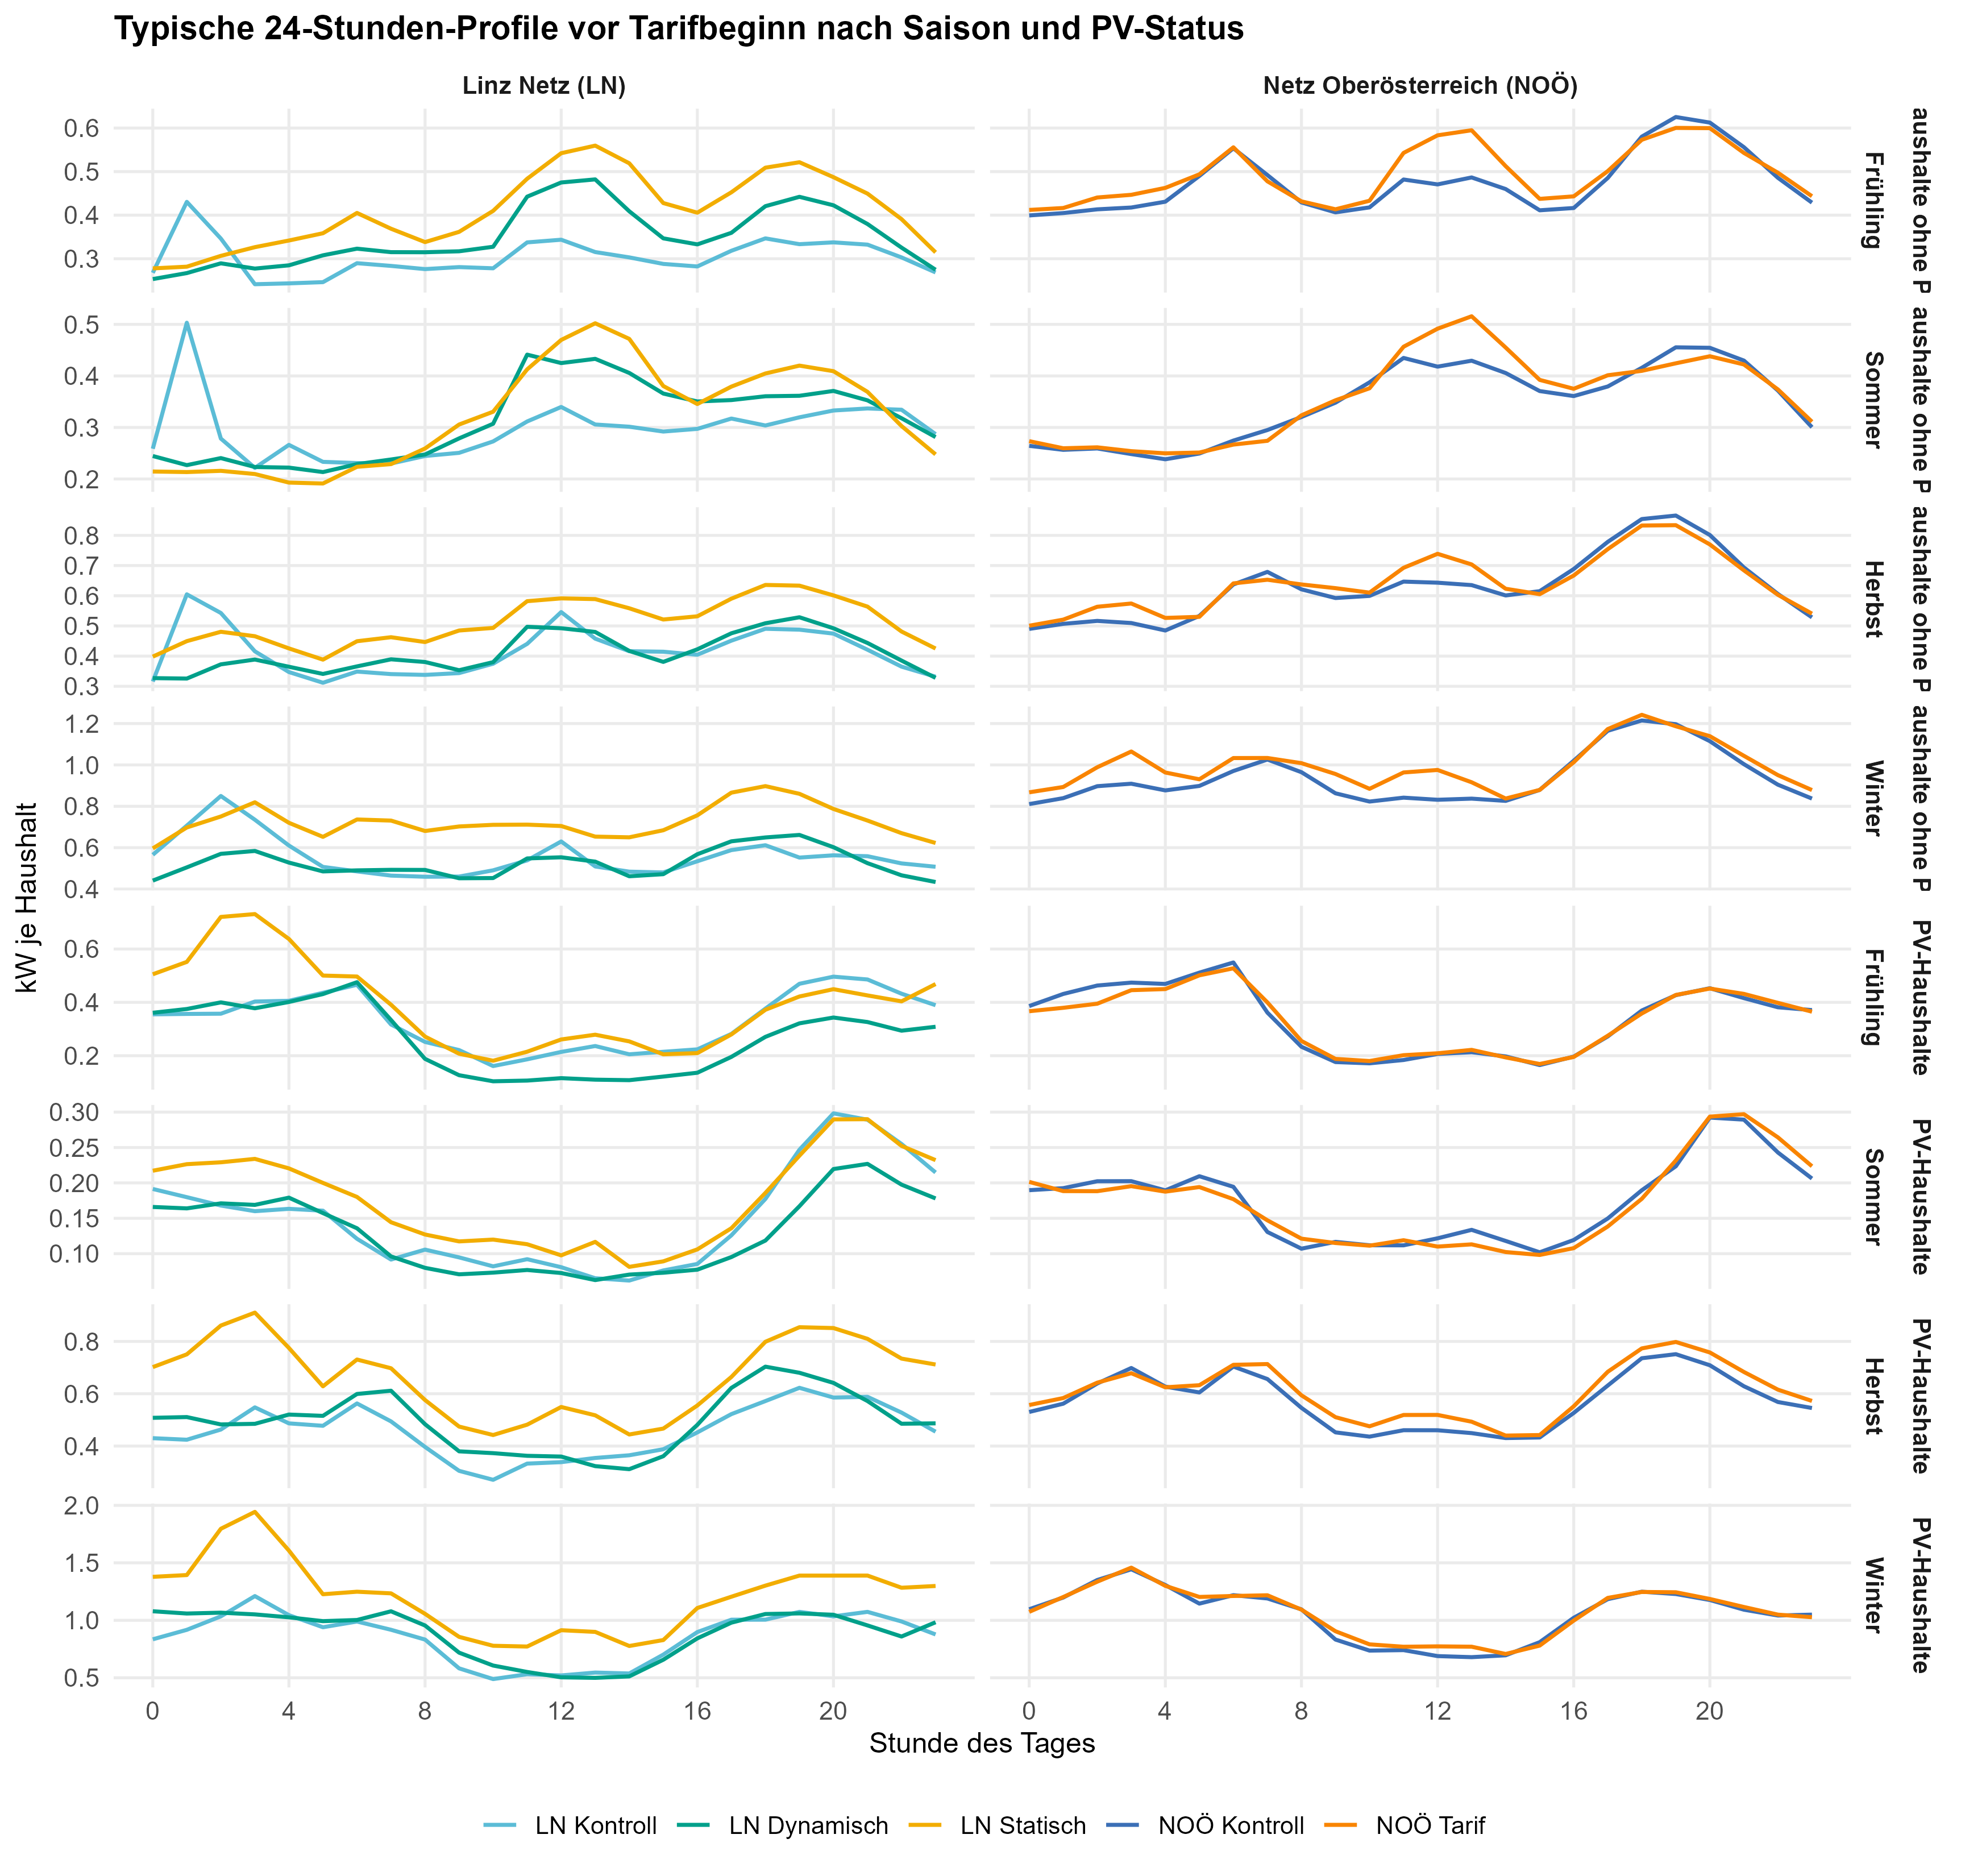
\includegraphics[width=1\linewidth]{paper/figures/report_fig05_seasonal_24h_profiles.png}
    \caption{Typische 24-Stunden-Profile des Netzbezugs vor Tarifbeginn nach Saison und PV-Status. Dargestellt ist der durchschnittliche stündliche Netzbezug je Haushalt.}
    \label{fig:report_seasonal_profiles}
\end{figure}

Für die folgenden deskriptiven Auswertungen ist diese Unterscheidung wichtig: In NOÖ beziehen sich die Signale auf Hoch-, Projekt-/Normal- und Niedrigtariffenster, während LN über Ausnahmefenster im Daily-Peak-Pricing funktioniert.

\subsection{Deskriptive Tagesprofile der drei NOÖ-Signalregime}

Die Abbildungen~\ref{fig:report_regime1_profile} bis \ref{fig:report_regime3_profile} zeigen den Netzbezug in den drei aufeinanderfolgenden NOÖ-Signalregimen. Sie dienen der deskriptiven Einordnung und sind nicht als kausale Effektschätzer zu verstehen. Insbesondere in den prognosebasierten Regimen~I und III hängen die ausgesendeten Tarifsignale von der lokalen Netzsituation ab.

\begin{figure}[H]
    \centering
    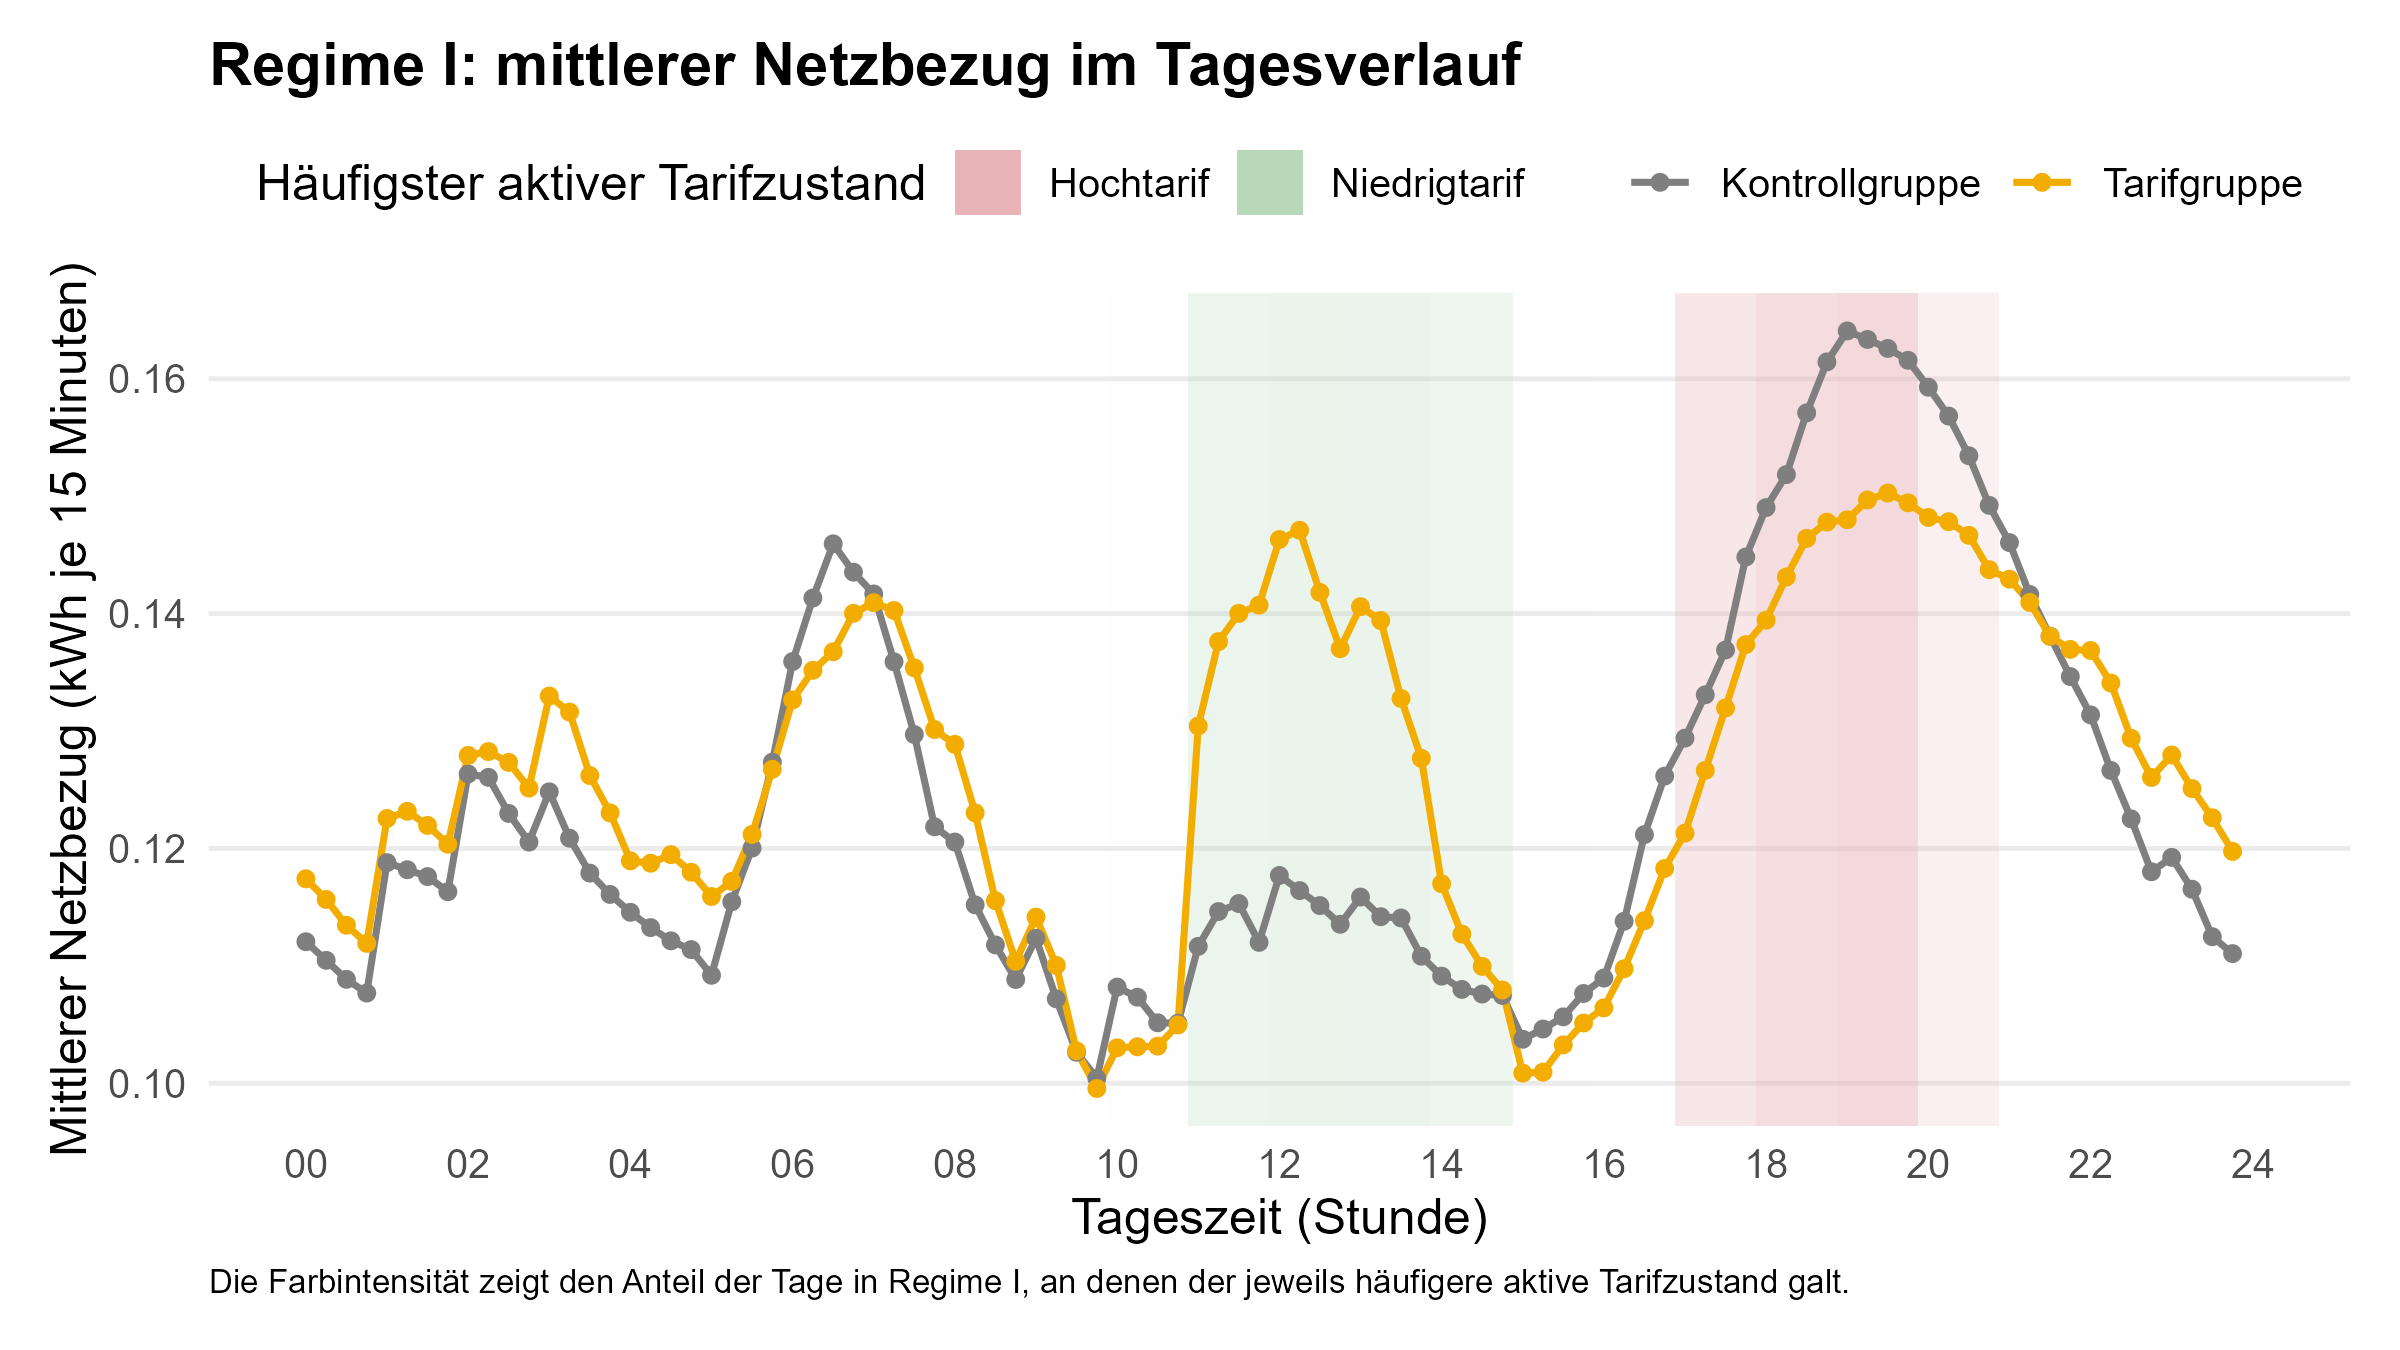
\includegraphics[width=0.92\linewidth]{paper/figures/report_fig06_regime1_tagesprofil.png}
    \caption{Mittlerer Netzbezug im Tagesverlauf in Regime~I. Die Hinterlegung zeigt den je Viertelstunde häufiger aktiven Niedrig- oder Hochtarif; eine intensivere Farbe steht für einen höheren Anteil der Regime-I-Tage mit diesem Signal.}
    \label{fig:report_regime1_profile}
\end{figure}

Regime~II verwendete einen durchgehend aktiven, binären Tarif mit rotierenden Signalblöcken. Ein über alle Haushalte gepooltes Tagesprofil würde daher unterschiedliche tatsächlich ausgesendete Signalfolgen vermischen. Abbildung~\ref{fig:report_regime2_profile} ordnet den Kontrollhaushalten stattdessen die beobachtete Signalfolge derselben Netzzone und Rotationsgruppe zu und zeigt für jede Viertelstunde die unbereinigte Differenz zwischen Tarif- und Kontrollgruppe.

\begin{figure}[H]
    \centering
    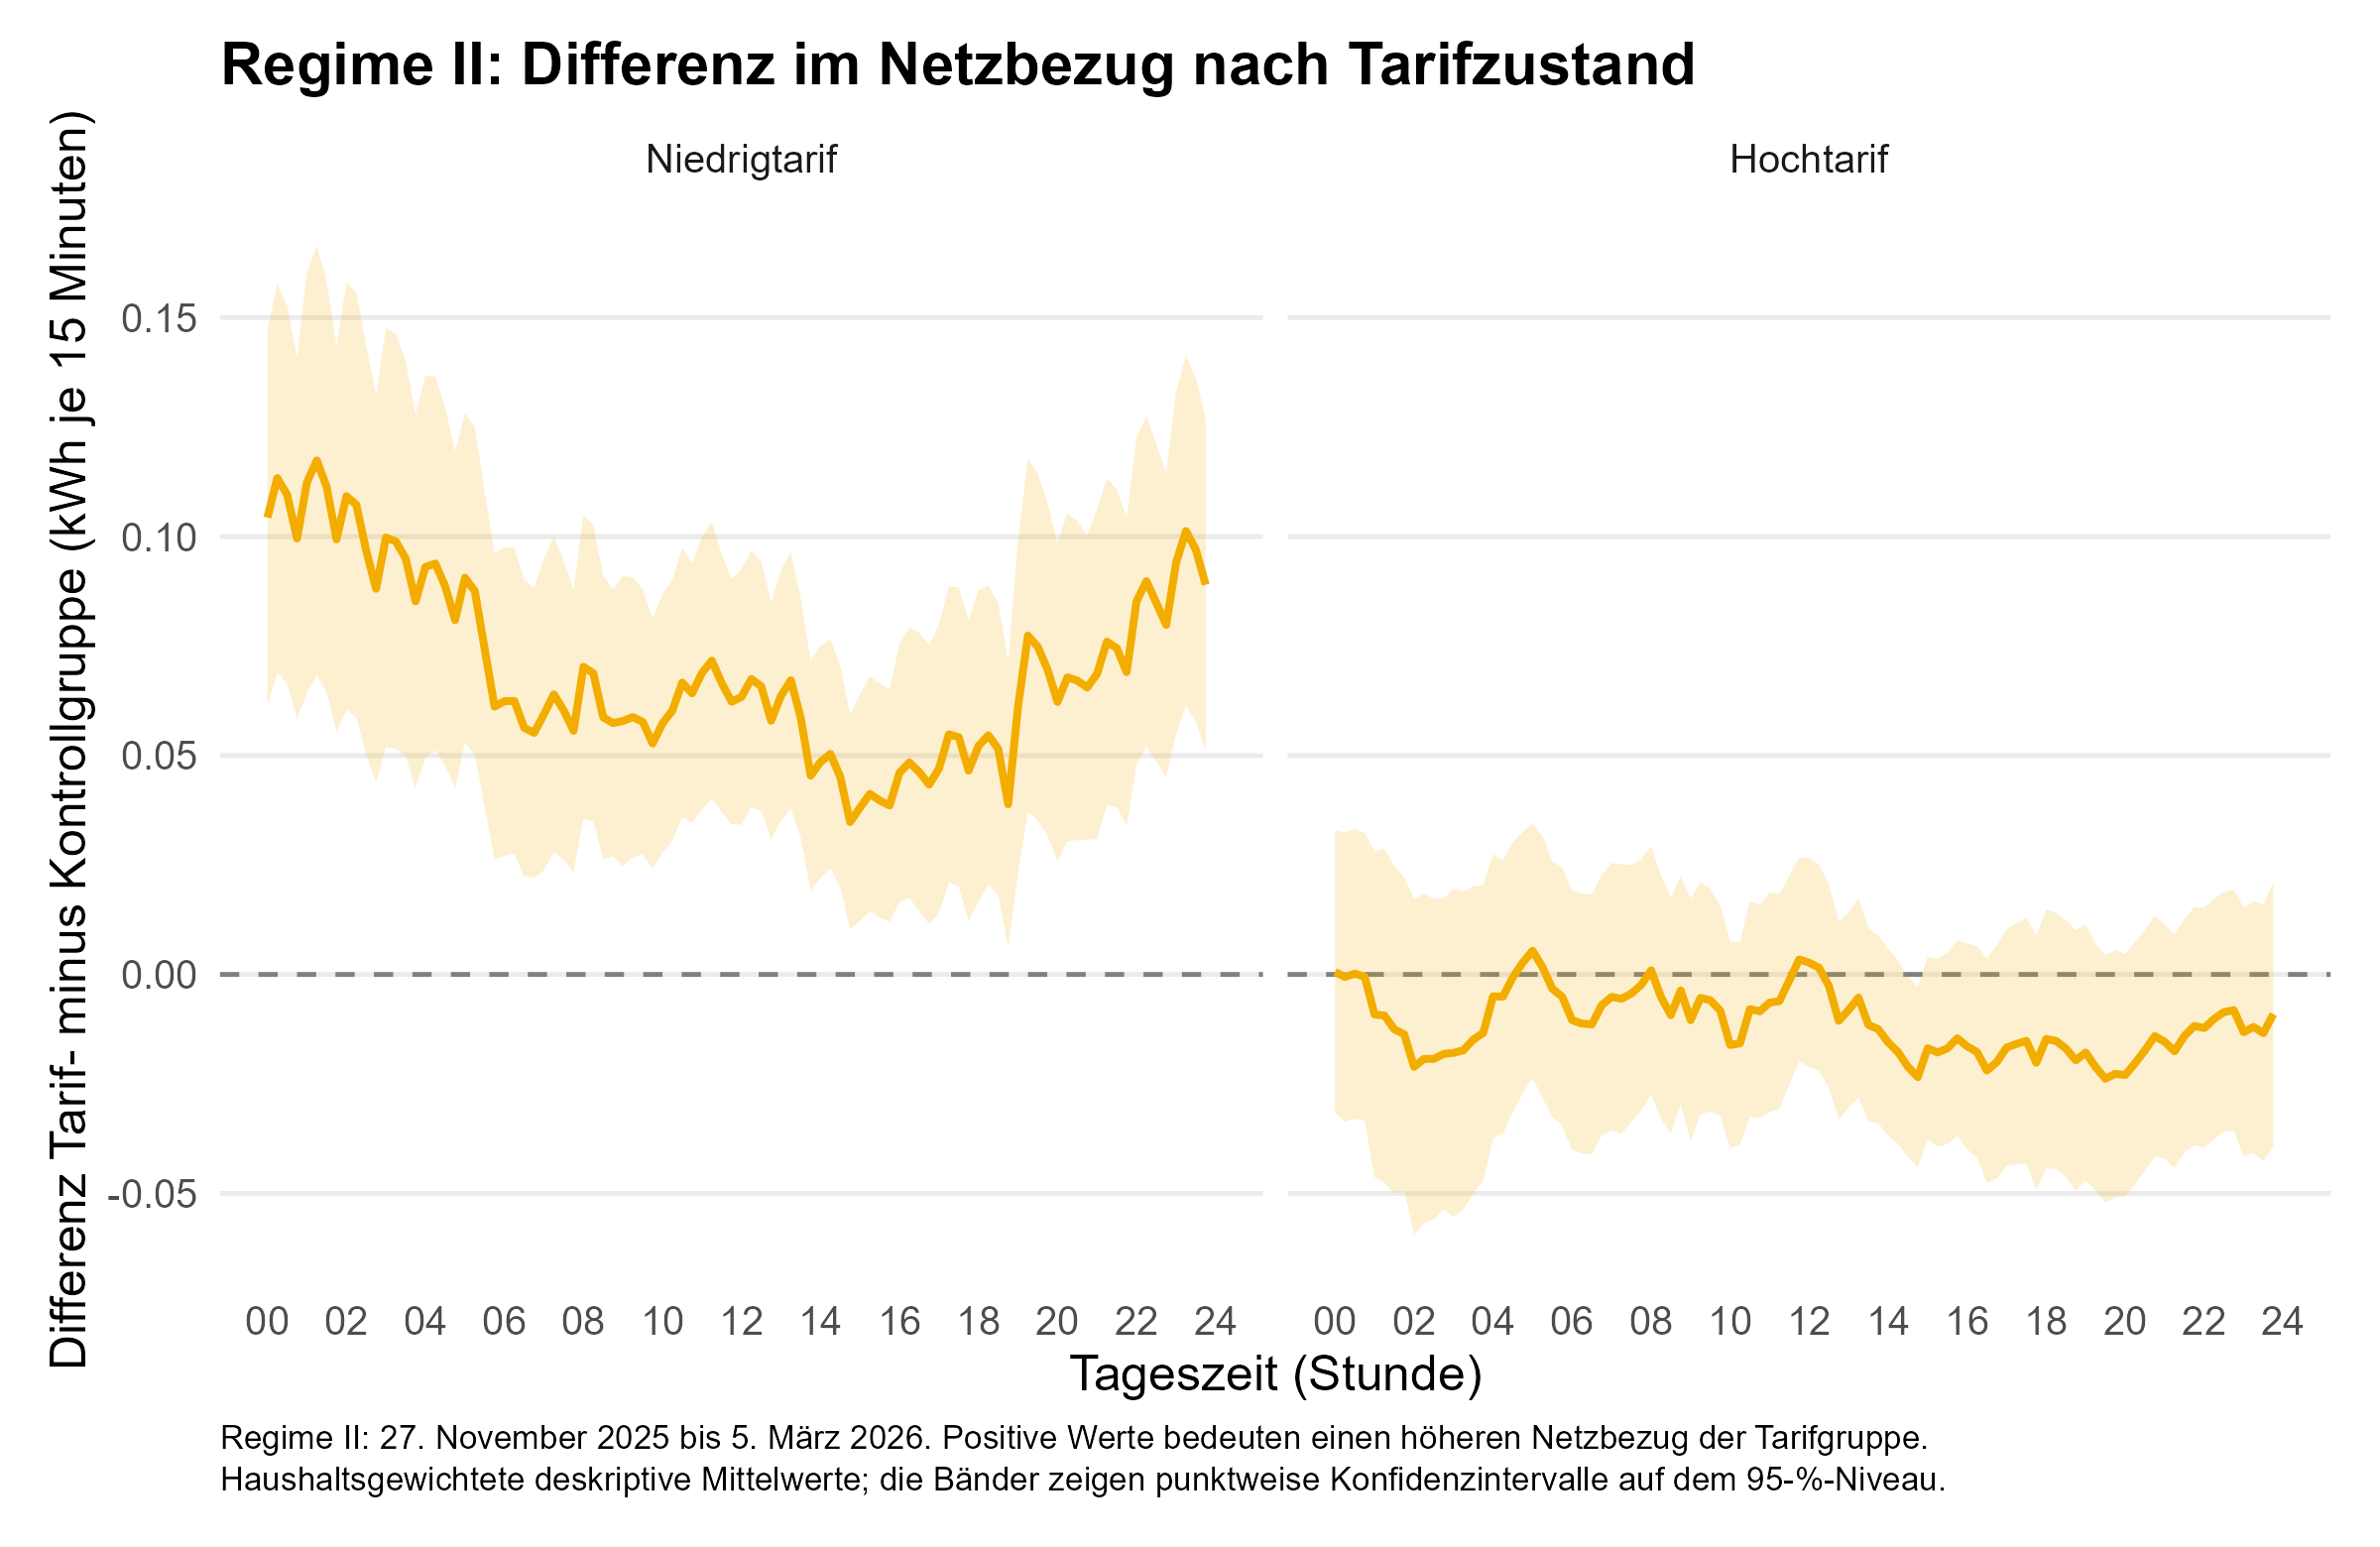
\includegraphics[width=0.96\linewidth]{paper/figures/report_fig07_regime2_tarifprofile.png}
    \caption{Unbereinigte Differenz im mittleren Netzbezug zwischen Tarif- und Kontrollgruppe nach Tarifzustand in Regime~II. Positive Werte bedeuten einen höheren Netzbezug der Tarifgruppe; die Bänder zeigen punktweise Konfidenzintervalle auf dem 95\%-Niveau über Haushalte.}
    \label{fig:report_regime2_profile}
\end{figure}

\begin{figure}[H]
    \centering
    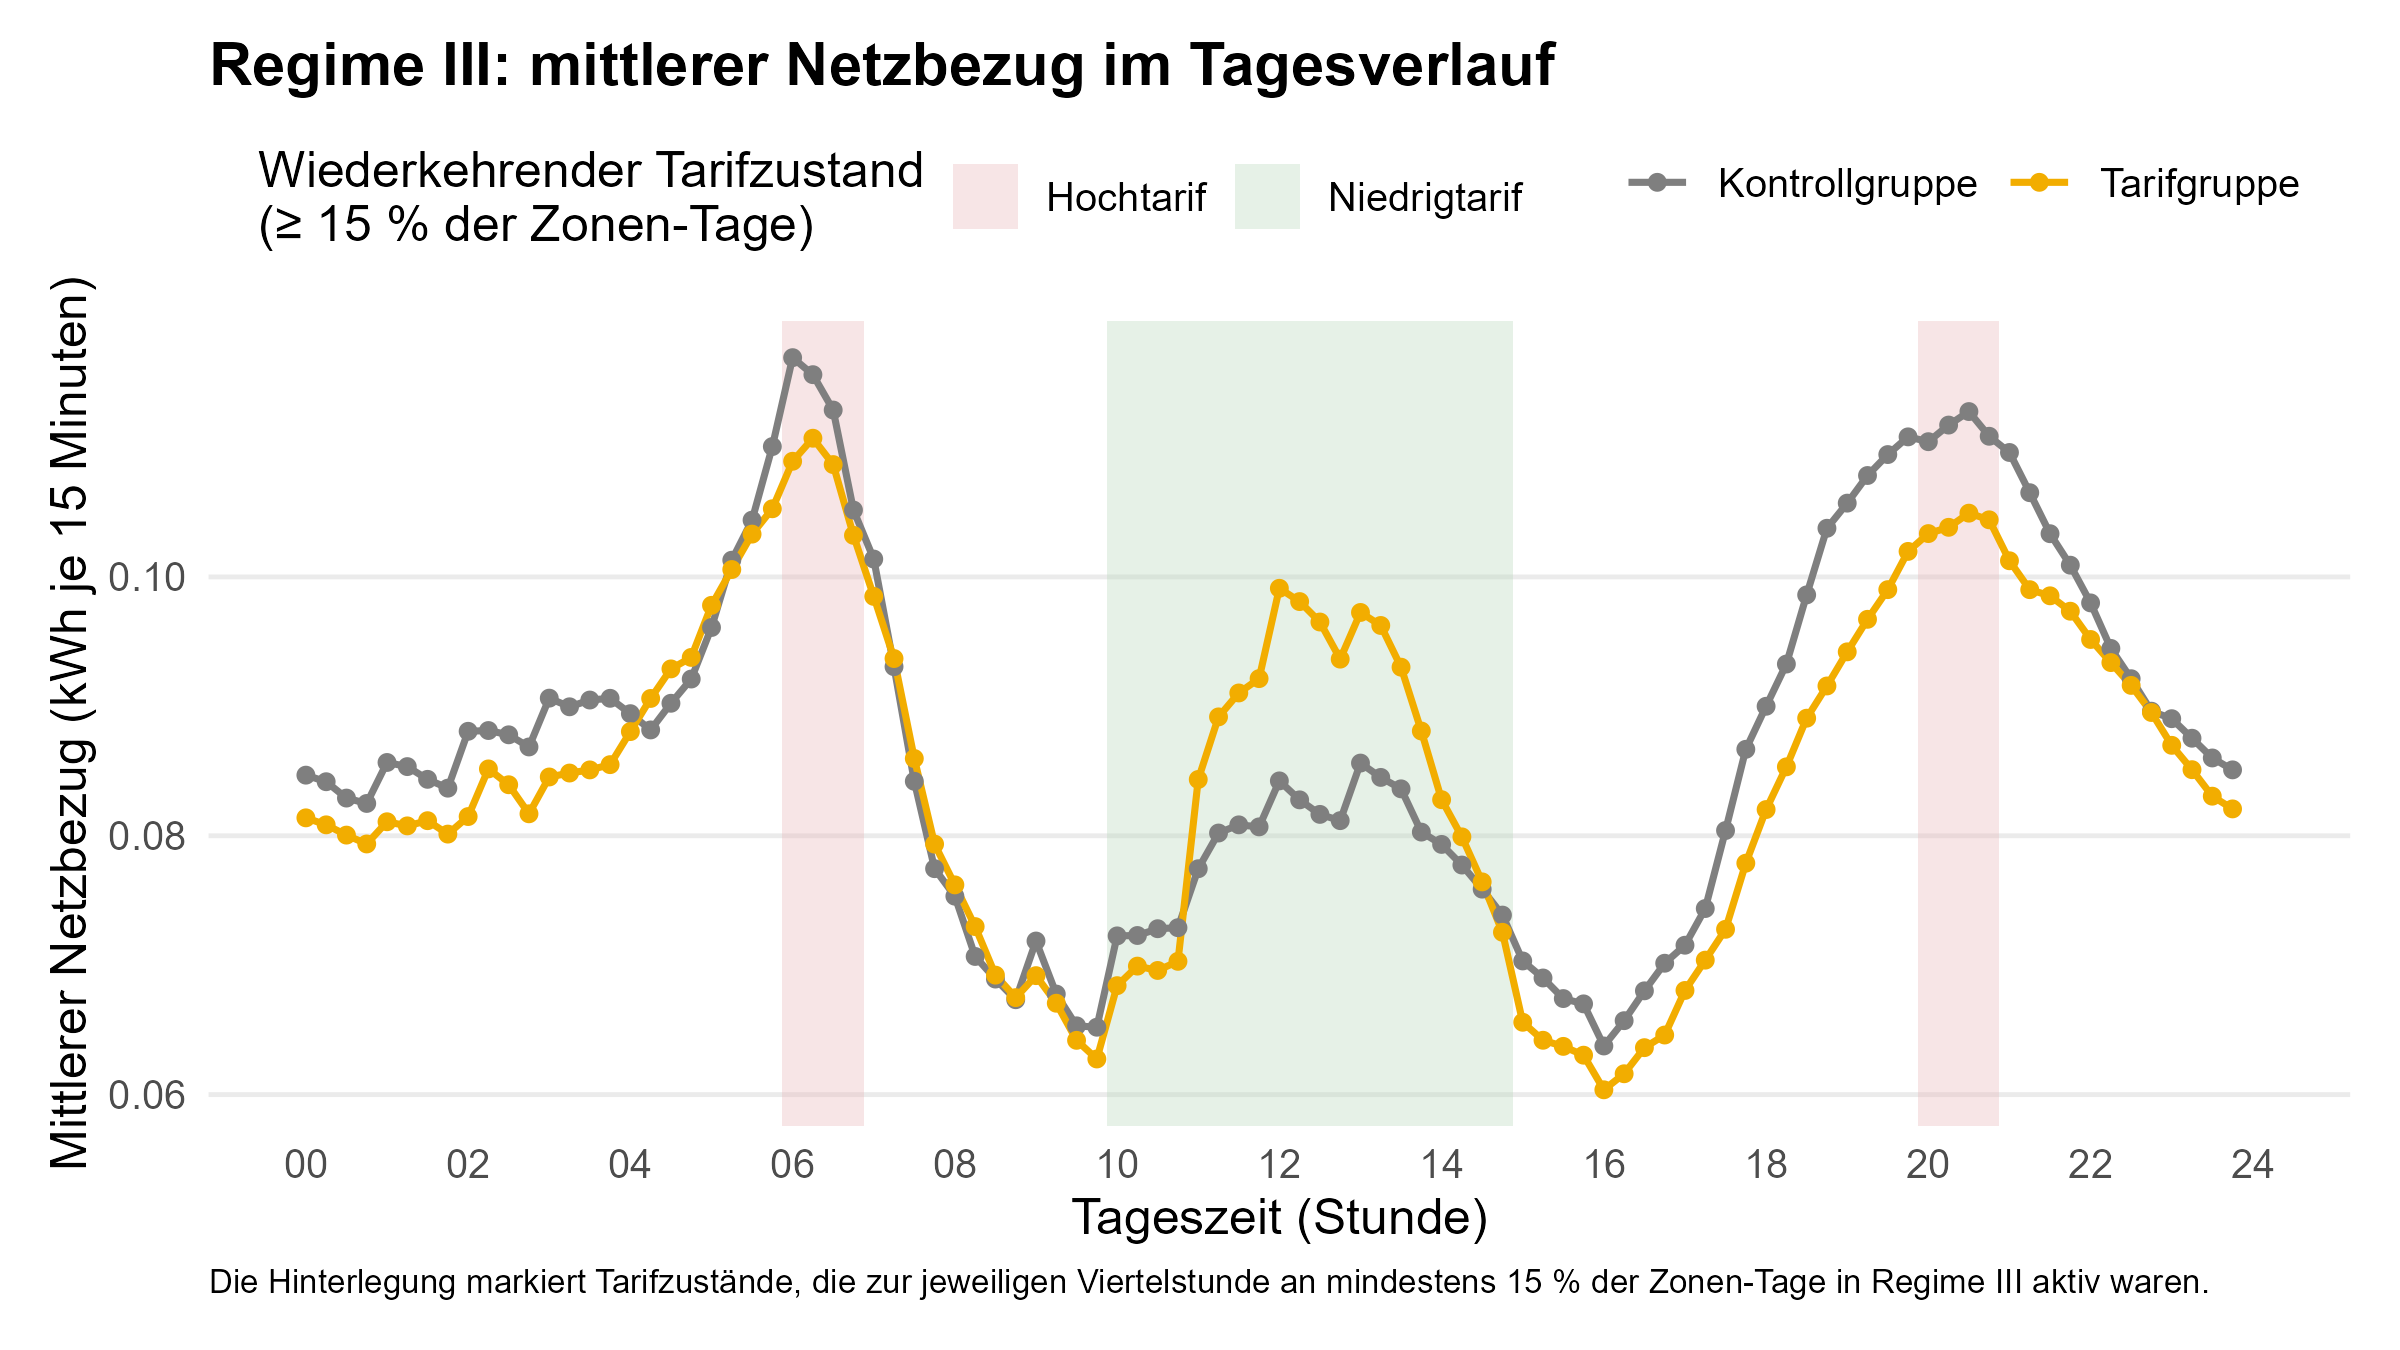
\includegraphics[width=0.92\linewidth]{paper/figures/report_fig08_regime3_tagesprofil.png}
    \caption{Mittlerer Netzbezug im Tagesverlauf in Regime~III. Die Hinterlegung markiert einen Tarifzustand nur dann, wenn er zur jeweiligen Viertelstunde an mindestens 15\% der Zonen-Tage aktiv war.}
    \label{fig:report_regime3_profile}
\end{figure}

\subsection{Parallele Trends in der Vorperiode}

Für die kausale Auswertung ist entscheidend, ob sich Tarif- und Kontrollgruppen vor Beginn der Intervention ähnlich entwickeln. Die Abbildungen~\ref{fig:report_pt_ln} und~\ref{fig:report_pt_noe} zeigen dazu den monatlichen Vorperiodenverlauf des täglichen Netzbezugs je Haushalt, getrennt nach Untersuchungsgruppe. Die Werte beruhen auf vollständigen Beobachtungstagen; die Bänder zeigen 95\%-Konfidenzintervalle über Haushalte, berechnet aus den monatlichen Haushaltsmitteln.

In LN verlaufen Kontrollgruppe und dynamischer Tarifarm über die gesamte Vorperiode nahezu deckungsgleich. Der statische Tarifarm liegt insbesondere in den Wintermonaten auf einem höheren Niveau, folgt aber demselben saisonalen Verlauf. Für die ökonometrische Analyse spricht dies dafür, den statischen Arm gesondert zu betrachten und Niveauunterschiede über Haushalts-Fixed-Effects aufzufangen. In NOÖ verlaufen Tarif- und Kontrollgruppe über die gesamte Vorperiode eng beieinander. Die formalen Event-Study-Tests im Ergebnisteil greifen diese deskriptiven Muster auf.

\begin{figure}[H]
    \centering
    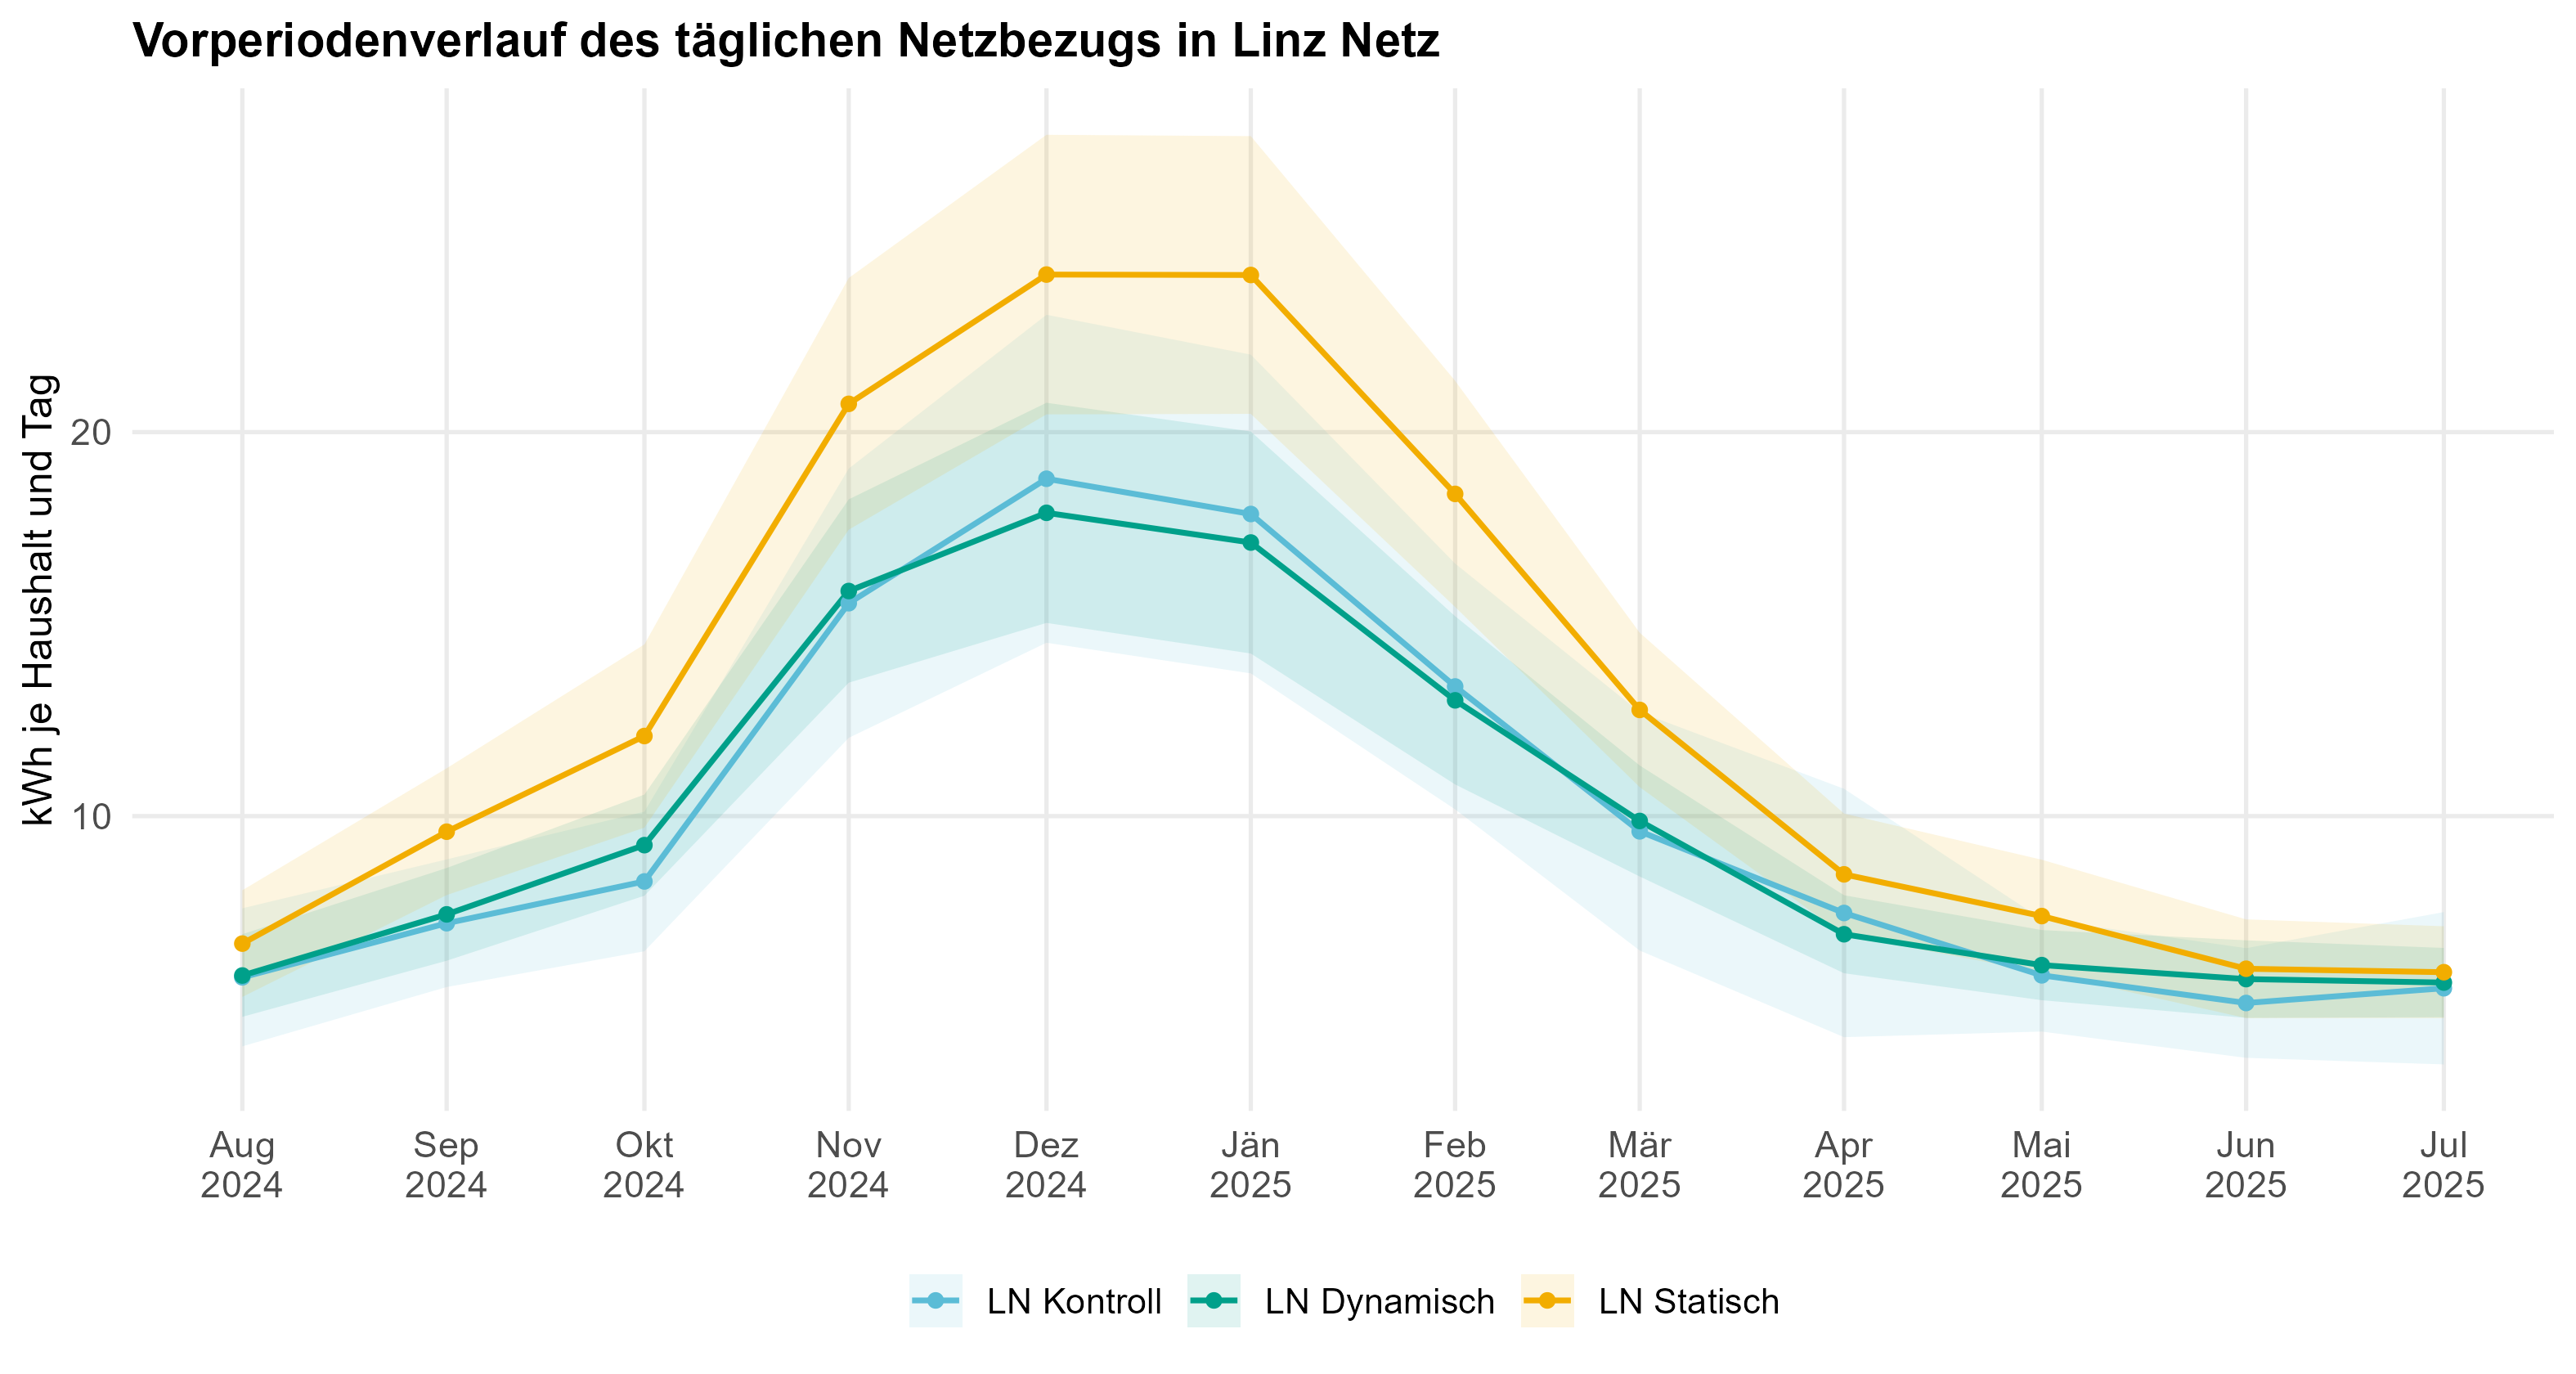
\includegraphics[width=1\linewidth]{paper/figures/report_pt_ln_monthly_consumption.png}
    \caption{Monatlicher Vorperiodenverlauf des täglichen Netzbezugs je Haushalt in Linz Netz nach Untersuchungsgruppe. Vollständige Beobachtungstage; die Bänder zeigen 95\%-Konfidenzintervalle über Haushalte.}
    \label{fig:report_pt_ln}
\end{figure}

\begin{figure}[H]
    \centering
    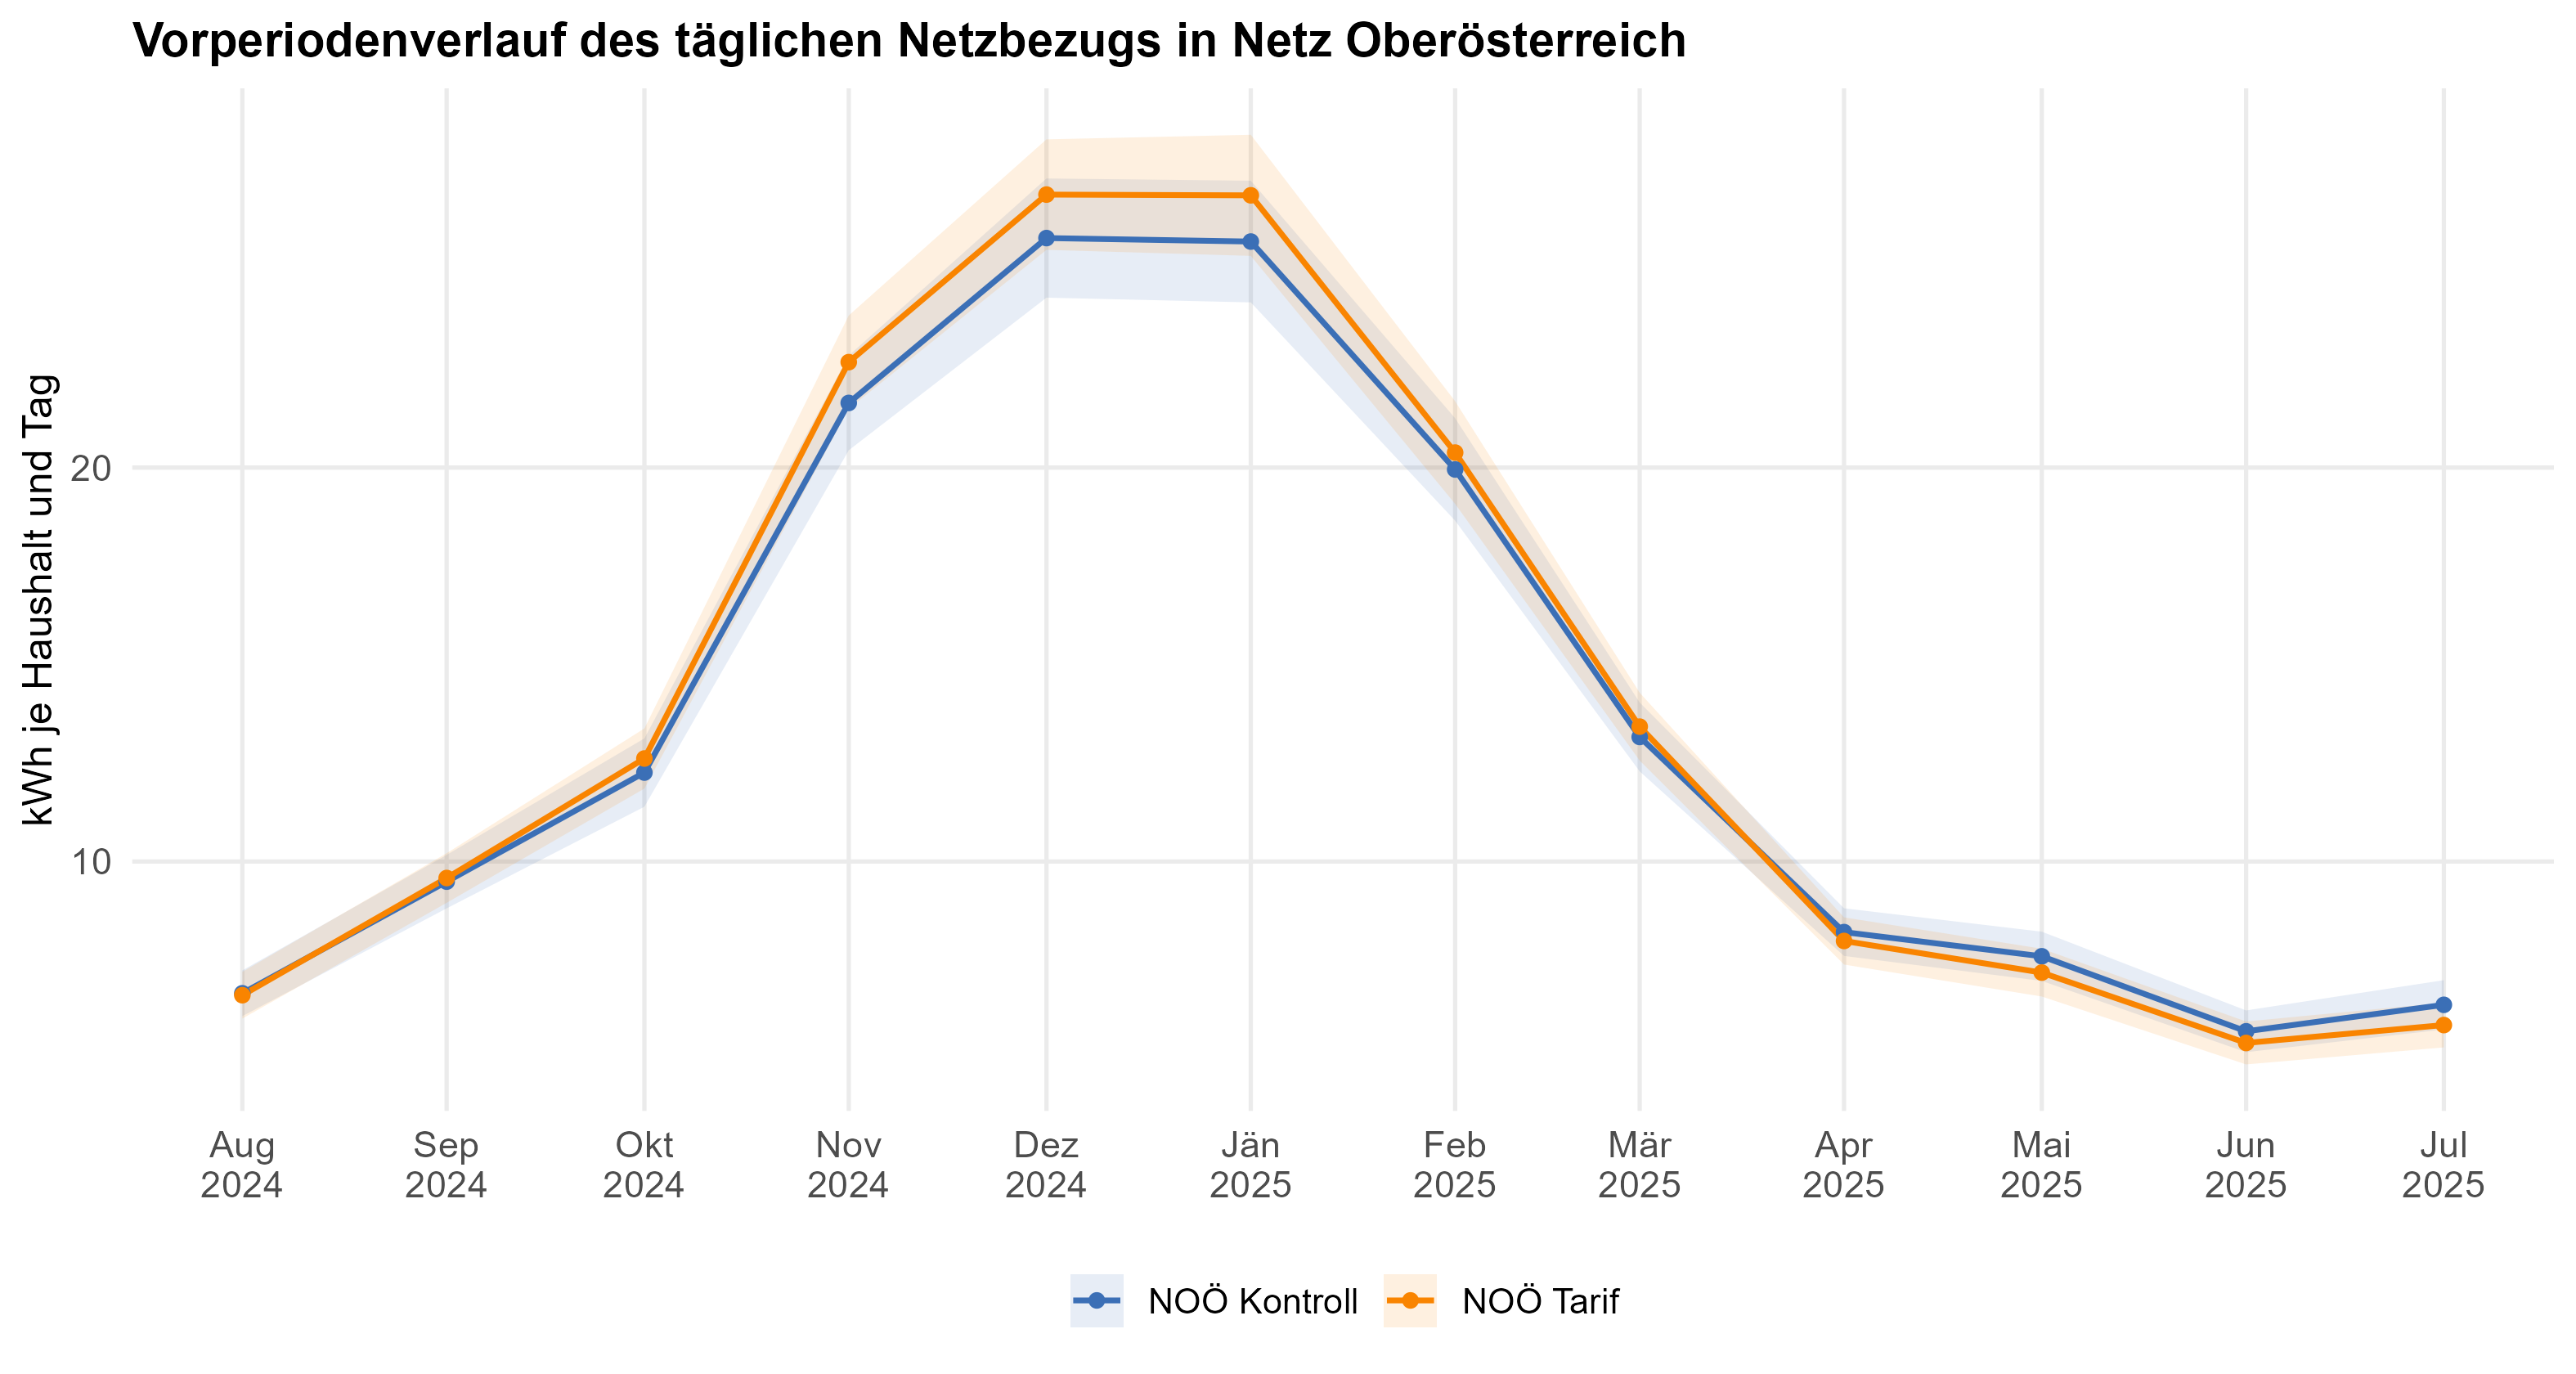
\includegraphics[width=1\linewidth]{paper/figures/report_pt_noe_monthly_consumption.png}
    \caption{Monatlicher Vorperiodenverlauf des täglichen Netzbezugs je Haushalt in Netz Oberösterreich nach Untersuchungsgruppe. Vollständige Beobachtungstage; die Bänder zeigen 95\%-Konfidenzintervalle über Haushalte.}
    \label{fig:report_pt_noe}
\end{figure}
